%% LyX 2.0.6 created this file.  For more info, see http://www.lyx.org/.
%% Do not edit unless you really know what you are doing.
\documentclass[english]{book}
\usepackage[latin9]{inputenc}
\usepackage{geometry}
\geometry{verbose,tmargin=1in,bmargin=1in,lmargin=1in,rmargin=1in}
\setcounter{secnumdepth}{3}
\setcounter{tocdepth}{3}
\usepackage{babel}
\usepackage{array}
\usepackage{varioref}
\usepackage{textcomp}
\usepackage{url}
\usepackage{graphicx}
\usepackage[unicode=true]
 {hyperref}

\makeatletter

%%%%%%%%%%%%%%%%%%%%%%%%%%%%%% LyX specific LaTeX commands.
\providecommand{\LyX}{\texorpdfstring%
  {L\kern-.1667em\lower.25em\hbox{Y}\kern-.125emX\@}
  {LyX}}
%% Because html converters don't know tabularnewline
\providecommand{\tabularnewline}{\\}

%%%%%%%%%%%%%%%%%%%%%%%%%%%%%% Textclass specific LaTeX commands.
\newenvironment{lyxcode}
{\par\begin{list}{}{
\setlength{\rightmargin}{\leftmargin}
\setlength{\listparindent}{0pt}% needed for AMS classes
\raggedright
\setlength{\itemsep}{0pt}
\setlength{\parsep}{0pt}
\normalfont\ttfamily}%
 \item[]}
{\end{list}}

%%%%%%%%%%%%%%%%%%%%%%%%%%%%%% User specified LaTeX commands.
\usepackage{hyperref}

\let\myUrl\url
\renewcommand{\url}[1]{(\myUrl{#1})}

\raggedbottom

\@ifundefined{showcaptionsetup}{}{%
 \PassOptionsToPackage{caption=false}{subfig}}
\usepackage{subfig}
\makeatother

\begin{document}

\title{Virtual California User Manual}


\author{� University of California, Davis\\
Version 1.0.0}


\date{\noindent \today}

\maketitle
\tableofcontents{}

\listoffigures



\part{Preface}


\chapter*{Preface}


\section*{About This Document}

This document is organized into three parts. Part I consists of traditional
book front matter, including this preface. Part II begins with an
introduction to Virtual California, the QuakeLib library, and their
capabilities then proceeds to the details of implementation. Part
III provides appendices and references for input and output files
and parameters.

The style of this publication is based on the Apple Publications Style
Guide \url{developer.apple.com/library/mac/documentation/UserExperience/Conceptual/APStyleGuide/APSG_2009.pdf},
as recommended by Python.org \url{www.python.org}. The documentation
was produced using \LyX{} \url{www.lyx.org} to facilitate the transformation
of files from one format to another. \LyX{} is a document processor
that encourages an approach to writing based on the structure of your
documents, not their appearance. It is released under a Free Software/Open
Source license.

Errors and bug fixes in this manual should be directed to the CIG
Mantle Convection Mailing List \url{cig-mc@geodynamics.org}.


\section*{Who Will Use This Document}

This documentation is aimed at two categories of users: scientists
who prefer to use prepackaged and specialized analysis tools, and
experienced computational Earth scientists. Of the latter, there are
likely to be two classes of users: those who just run models, and
those who modify the source code. Users who modify the source are
likely to have familiarity with scripting, software installation,
and programming, but are not necessarily professional programmers.

The manual was written for the usage of Virtual California on a variety
of different platforms. Virtual California has run on shared memory
computers (Sun, Hewlett-Packard, SGI, and IBM), commercial distributed
memory machines (Intel and Cray/SGI), clusters (including machines
on NSF XSEDE), Linux PCs and Mac OS X desktops. 


\section*{Citation}

Computational Infrastructure for Geodynamics (CIG) is making this
source code available to you in the hope that the software will enhance
your research in geophysics, and probabilistic seismic hazard analysis.
The underlying C++ code for the Greens function calculations, stress
evolution, simulation framework, and the QuakeLib library and associated
Python bindings and testing framework were donated to CIG in December
of 2012. A number of individuals have contributed a significant portion
of their careers toward the development of Virtual California. It
is essential that you recognize these individuals in the normal scientific
practice by citing the appropriate peer reviewed papers and making
appropriate acknowledgements. 

The Virtual California development team asks that you cite both of
the following:
\begin{itemize}
\item Heien, E.M., Sachs, M.K., \char`\"{}Understanding Long-Term Earthquake
Behavior through Simulation,\char`\"{} Computing in Science and Engineering,
pp. 10-20, Sept.-Oct., 2012 
\item Sachs, M.K., Heien, E.M., Turcotte, D.L., Yikilmaz, M.B., Rundle,
J.B., Kellogg, L.H. ''Virtual California Earthquake Simulator''
Seismological Research Letters, November/December 2012, v. 83, p.
973-978, doi:10.1785/0220120052
\end{itemize}
The developers also request that in your oral presentations and in
your paper acknowledgements that you indicate your use of this code,
the authors of the code, and CIG \url{geodynamics.org}.


\section*{Support}

Support for this work and researchers was provided by multiple sources.
This work was supported by the National Aeronautics and Space Administration
(NASA) grant number NNX08AF69G, JPL subcontract number 1291967, and
NASA Earth and Space Science Fellowship number NNX11AL92H. Support
was also given by the Southern California Earthquake Center (SCEC).
SCEC is funded by the National Science Foundation Cooperative Agreement
EAR-0529922 and U.S. Geological Survey (USGS) Cooperative Agreement
07HQAG0008. This work also used the Extreme Science and Engineering
Discovery Environment (XSEDE), which is supported by National Science
Foundation grant number OCI-1053575. Any opinions, findings, and conclusions
or recommendations expressed in this material are those of the authors
and do not necessarily reflect the views of the National Science Foundation.


\section*{Conventions}

Throughout this documentation, any mention of ``username'' is meant
to indicate the user, meaning you should substitute your account name
in its place.


\part{Chapters}


\chapter{Introductions}

Virtual California is a boundary element code designed to investigate
long term fault system behavior and interactions between faults through
stress transfer. It is released under the MIT Public License (see
Appendix \ref{chap:License}). The core code is written in C++ and
can be run on a variety of parallel processing computers, including
shared and distributed memory platforms. To allow increased functionality
including development of other simulators, analysis scripts, and visualization
tools, some key components of Virtual California have been placed
in the QuakeLib library which can be called from C/C++ programs or
Python scripts.


\section{About Virtual California}

Virtual California is a boundary element code that performs simulations
of fault systems based on stress interactions between fault elements
to understand long term statistical behavior. It performs these simulations
using a model of faults embedded in a homogeneous elastic half space
with arbitrary dips and rakes.

The code performs calculation assuming linear stress increase in the
long term based on element-element interaction calculations governed
by Okada's implementation of Green's functions. During the rupture
(earthquake) phase elements may fail and release stress based on a
combination of static and dynamic stress thresholds. The behavior
of the system is determined by interactions between elements from
the Green's function and the stress release from elements during events.
More detail about the equations and physics of the simulation is described
in Section \ref{sec:Governing-Equations}.


\section{History}

Virtual California (abbreviated VC) started as a limited simulation
model for distributed seismicity on the San Andreas and adjacent faults
in southern California, developed by Rundle \cite{Rundle:1988bj}
in Fortran. This model included stress accumulation, release and interactions
between faults to investigate earthquake dynamics in southern California.
The model was updated in the early to mid-2000s \cite{2001PhRvL..87n8501R,Rundle2002gem,Rundle2006vc}
to include major strike-slip faults in California and was named Virtual
California. This model and simulation was used to examine recurrence
time statistics on California faults by Yakovlev \cite{2005AGUFMNG21A..03Y},
where it was concluded that the return times on a fault is well approximated
by a Weibull distribution.

In 2010 Virtual California was rewritten by Eric Heien in C++ to have
a more modular simulation framework and add support for multiprocessor
simulation using OpenMP and/or MPI. The fault model in Virtual California
was also more cleanly separated from the fundamental stress calculation
to allow simulation of other fault systems, including the Nankai trough
in Japan \cite{2010PhDT}. Additional features were also added, including
a branching aftershock sequence (BASS) model simulation of aftershocks
\cite{npg-18-955-2011}, improved stress Green's function calculations,
more sophisticated rupture propagation, and support of parallel HDF5
output. Virtual California was also used in an effort by the Southern
California Earthquake Center to unify and compare the results from
several earthquake simulators \cite{TullisNovember/December}.

In 2011 and 2012, core components of Virtual California were separated
into the QuakeLib library and used to create analysis and visualization
tools. Improvements to simulation performance were also developed,
including speculative execution for rupture propagation and a Barnes-Hut
style approximation scheme for the Green's functions.


\section{About QuakeLib\label{sec:About_quakelib}}

QuakeLib is a C++ library containing key mathematics, geophysics and
I/O functionality related to earthquake simulation and result analysis.
QuakeLib is currently distributed with and is used by Virtual California,
though it can be compiled and installed by itself on a machine. More
specifically, QuakeLib contains 1) functions to read, write and validate
fault models and earthquake catalogs in the EqSim format, 2) C++ classes
to represent and access these models and catalogs, 3) C++ classes
to represent faults and associated fault parameters as well as functionality
related to the faults, 4) C++ classes and functions to perform vector
mathematics and unit/geographic conversions related to modeling, 5)
functions to evaluate stress and displacement fields based on Okada's
equations \cite{Okada01041992} given a rectangular fault or point
source.

QuakeLib is also written to support extension to other scripting languages
through the use of the Simplified Wrapper and Interface Generator
(SWIG) \cite{Beazley:1996:SEU:1267498.1267513}. Currently this supports
wrapping the QuakeLib library in a Python interface though additional
scripting languages can be easily added. The scripting extension allows
researchers to write analysis and visualization scripts based on the
same equations and data formats as the simulation. The Python interface
is also used as the basis for a testing framework to ensure that any
changes made to the code do not affect the scientific results and
that computations on different platforms yield the same results within
a specified tolerance.


\chapter{VC Simulation Components and Governing Equations\label{sec:Governing-Equations}}

There are three major components that make up Virtual California:
a fault model, a set of quasi-static interactions (Green\textquoteright{}s
functions), and an event model. In spite of the name, the only component
of Virtual California that is specific to California is the fault
model. This model can be changed to any physically realistic model
and still correctly work with the simulation physics and event model. 

The first three sections cover the main components of a VC simulation,
the fourth section describes the simulation flow, and the last section
gives a visual tour of the QuakeLib module's functionality.


\section{Fault Model\label{sec:Fault_model}}

The basic components of the fault model are the fault elements and
their parameters. Any fault system, specified by a trace file listing
the latitude and longitude of each vertex along the traces, is split
up into the functional members of a Virtual California simulation,
the fault elements. The resolution of the fault system will determine
the total number of elements, and each element's parameters determine
the local fault geometry and motion.

Each element in the model is given a constant back-slip velocity along
a fixed rake vector and a failure stress. The rake vector always lies
in the plane of the element. The failure stresses, which are also
required for the model, are derived from paleoseismic event recurrence
times.


\subsection{Current California Fault Model}

The full model for the California fault system that we currently use
is based on the ALLCAL2 fault model, shown in Figure \ref{fig:UCERF2_google_earth}.
A detailed description of the ALLCAL2 model is at \url{http://scec.usc.edu/research/eqsims/documentation.html},
and description of file formats is in \cite{Barall01112012}. The
model includes 181 fault sections roughly corresponding to known faults
in California, with some faults modeled by multiple sections. Each
fault section is meshed into square elements that are roughly 3 km
\texttimes{} 3 km, for a total of 14,474 elements. In the present
version of our model, the creeping section of the San Andreas fault
is removed. This section produces many events, slowing the simulation
down considerably. 

\begin{figure}[th]
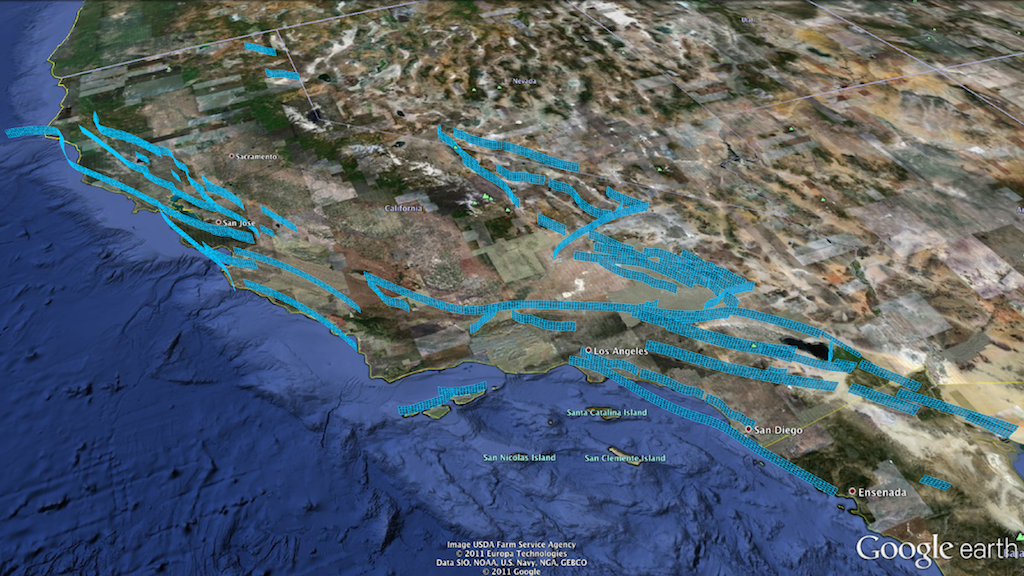
\includegraphics[width=1\textwidth]{graphics/UCERF2_faults_GoogleEarth}\caption{California fault system based on UCERF2, meshed into fault elements
and shown above ground.\label{fig:UCERF2_google_earth}}
\end{figure}



\subsection{Model Parameters and Initial Conditions}

Virtual California currently requires that the user specify the fault
geometry and the stress parameters on each element then run the simulation
based on this. These parameters are briefly described in the following
section, and explicit example fault models are constructed in chapter
\ref{cha:Cookbooks}.


\subsection{Setting Fault Parameters and Building a Fault Model\label{sec:define_mesh_faults}}

VC treats a system of faults as multiple planar elements embedded
in a flat homogeneous halfspace. To run Virtual California the first
step is to define a fault system using a set of traces. Each trace
describes the points along a given fault closest to the surface as
well as fault characteristics at each trace point, such as long term
velocity, dip angle, rake angle, depth, etc. Details about the trace
file format are shown in Appendix \ref{sec:Trace-File-Format}.

In this example we look at the earthquake cycle and rupture mechanics
on a single 12 km square fault. For simplicity, the trace of this
fault runs eastward for 12km starting from latitude/longitude (0,0)
and ending at latitude/longitude (0,0.1078). The definition of this
fault is in the file examples/fault\_traces/single\_fault\_trace.txt
and is also shown below.
\begin{lyxcode}
\#~fault\_id:~ID~number~of~the~parent~fault~of~this~section

\#~num\_points:~Number~of~trace~points~comprising~this~section

\#~section\_name:~Name~of~the~section

0~2~One\_Element\_Example

\#~latitude:~Latitude~of~trace~point

\#~longitude:~Longitude~of~trace~point

\#~altitude:~Altitude~of~trace~point~(meters)

\#~depth\_along\_dip:~Depth~along~dip~(meters)

\#~slip\_rate:~Slip~rate~at~trace~point~(centimeters/year)

\#~aseismic:~Fraction~of~slip~that~is~aseismic~at~point

\#~rake:~Fault~rake~at~trace~point~(degrees)

\#~dip:~Fault~dip~at~trace~point~(degrees)

\#~lame\_mu:~Lame's~mu~parameter~at~trace~point~(Pascals)

\#~lame\_lambda:~Lame's~lambda~parameter~at~trace~point~(Pascals)

0~0~0~12000~1~0~180~90~3e+10~3.2e+10

0~0.1078~0~12000~1~0~180~90~3e+10~3.2e+10~
\end{lyxcode}
The first non-comment line in this file gives the fault ID, number
of trace points, and fault name. In this example, the fault is named
\char`\"{}One\_Fault\_Example\char`\"{}. The remaining non-comment
lines give the fault characteristics at each trace point. This file
defines two trace points, the first at latitude/longitude (0,0) and
the second at (0, 0.1078), with both at altitude 0. At each point
the fault extends 12,000 meters down and has a slip rate of 1 cm/year
with 0 aseismicity. The fault is right lateral strike slip (rake of
180\textdegree{}, dip of 90\textdegree{}). The Lam� parameters of
$\mu=3e10$ and $\lambda=3.2e10$ indicate the material properties
of the fault.

Given this fault definition we can create a mesh which fits within
the fault dimensions. Each fault is meshed by specifying the fault
trace file in the format described above, and a fault element size.
Currently all fault elements in Virtual California are square though
future versions will allow triangulare elements. Furthermore, all
elements of a single fault are meshed at the same resolution. This
means that if the meshing resolution is not a perfect multiple of
the trace length or depth at a given point, the meshed elements will
not completely cover the trace.

Figure \ref{fig:trace_mesh_example} shows this for an example fault
trace consisting of 4 trace points, where the fault trace is represented
by a dashed line and the meshed elements represented by red segments.
Figure \ref{fig:exact_trace_mesh} shows the meshed model on this
fault with elements that match the lengths between the trace points.
Because the distance between trace points is exactly a multiple of
the element size, the meshed elements exactly cover the fault trace.
Figure \ref{fig:offset_trace_mesh} shows the same fault trace with
smaller meshed elements. The first element follows the trace but the
second element deviates in order to fit the meshed element along the
trace. In practice, this discrepancy is usually not a big issue because
fault traces are not significantly non-linear. Also, as elements become
smaller relative to the distance between trace points this discrepancy
becomes smaller.

\begin{figure}
\subfloat[\label{fig:exact_trace_mesh}Using an element size that exactly aligns
with the trace, the generated elements will exactly follow the trace.]{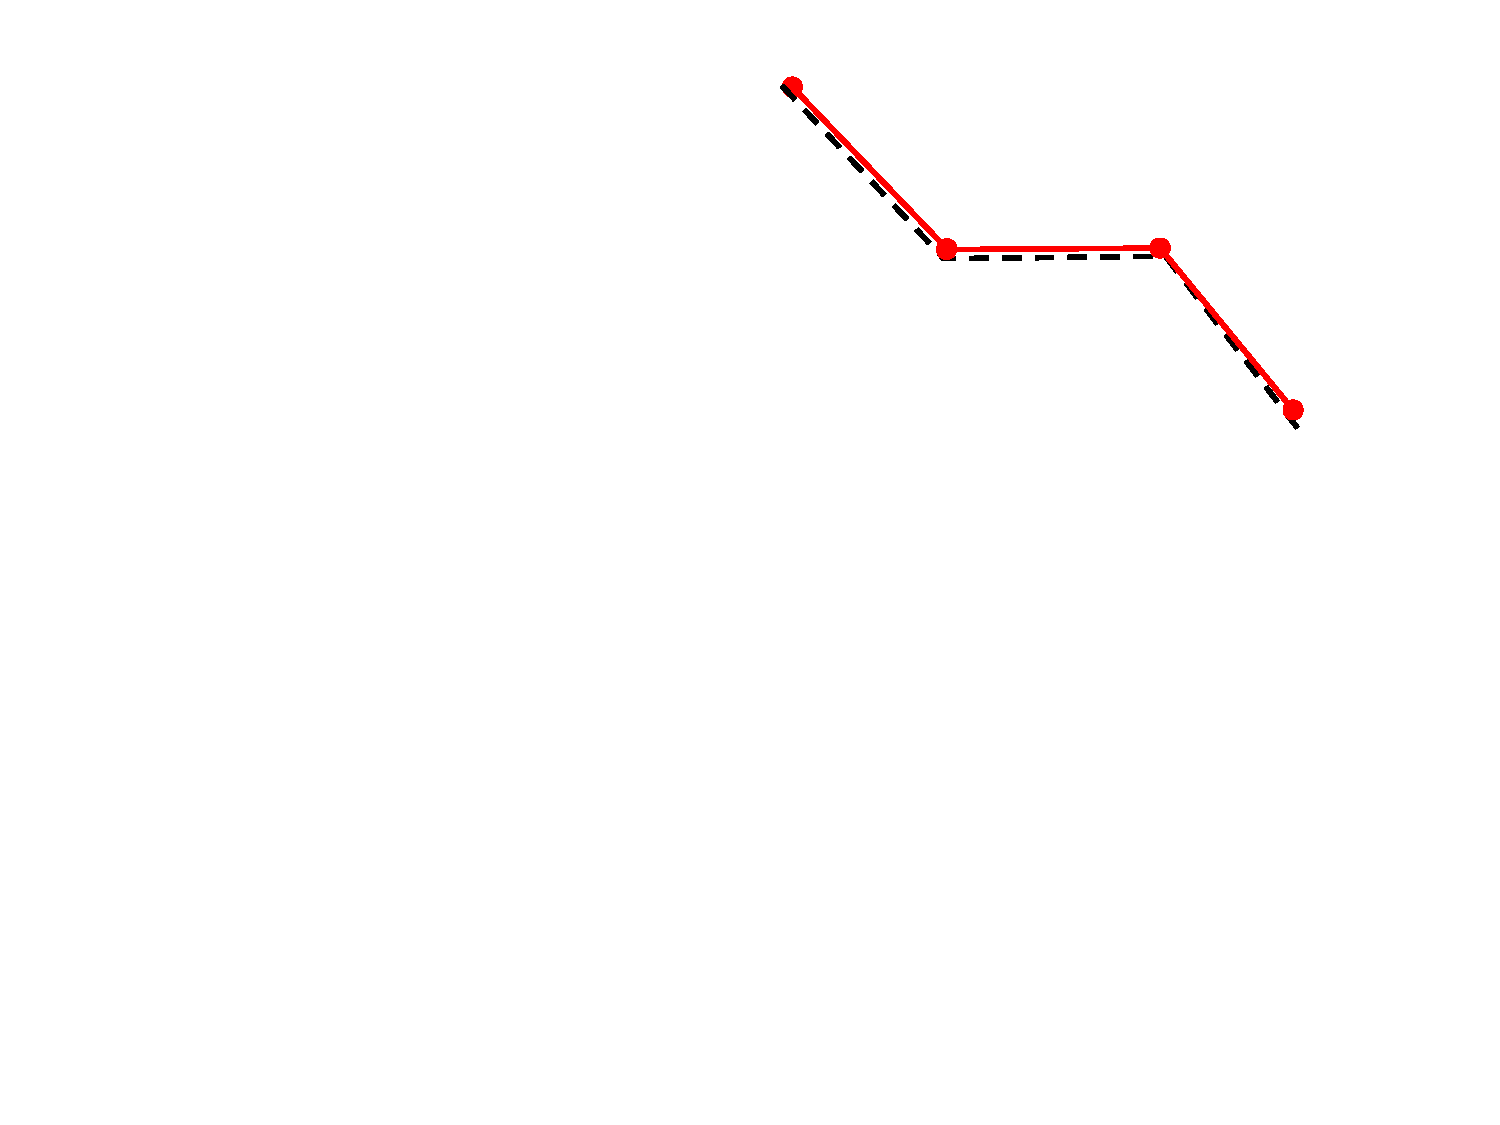
\includegraphics[width=0.48\textwidth]{graphics/FaultTrace3elem}}\hfill{}\subfloat[\label{fig:offset_trace_mesh}A slightly smaller element size results
in a mesh that does not exactly follow the trace.]{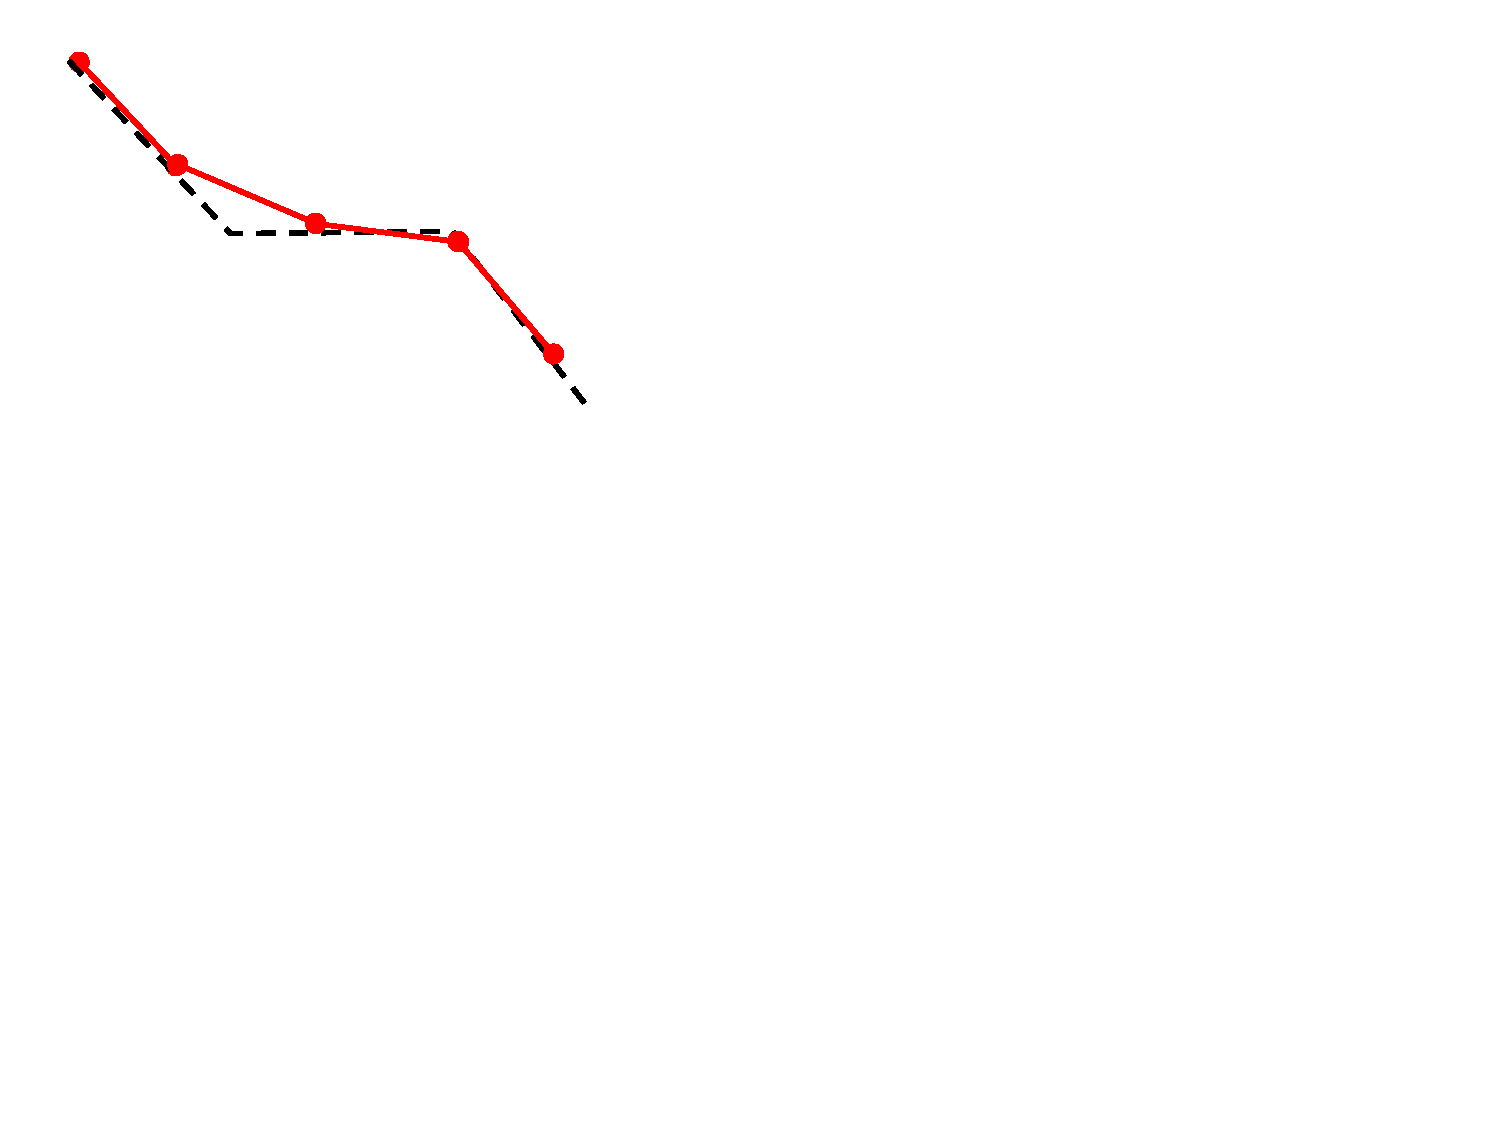
\includegraphics[width=0.48\textwidth]{graphics/FaultTrace4elem}

}

\caption{\label{fig:trace_mesh_example}An example of how element size will
affect the tracking of the mesh along a fault trace.}
\end{figure}


When creating a meshed element along a fault trace it is necessary
to assign characteristics to the element such as slip rate, aseismic
slip, rake, dip, and Lam� parameters. These are determined by linear
interpolation of the fault trace values at the midpoint of the meshed
element.

The use of linear interpolation for values between fault trace points
also means that if the meshed elements are larger than the distance
between fault trace points and there is significant variation between
trace point characteristics, then this variation may be lost during
the meshing process. In general it is recommended to use an element
size smaller than the smallest distance between fault trace points
unless there are memory or computing constraints. In the event that
the meshing process skips a trace point because of overly large element
size, a warning will be output. Appropriate element size is further
discussed in Section \ref{sec:element_size_discussion}. The meshing
program and related parameters are described in Section \ref{sec:building_faults}.

\begin{figure}
\subfloat[\label{fig:mesh6km}Example 12km x 12km fault meshed at 6km resolution
giving 2 x 2 = 4 total elements.]{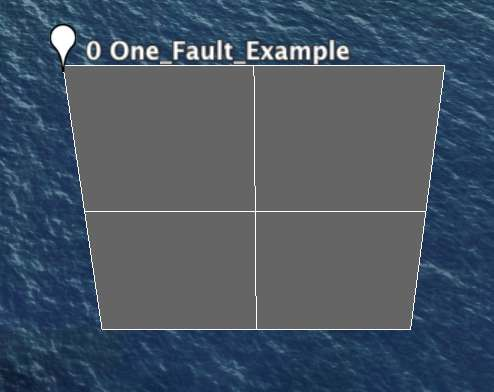
\includegraphics[height=5cm]{graphics/single_fault_6k}}\hfill{}\subfloat[\label{fig:mesh4km}Example 12km x 12km fault meshed at 4km element
resolution giving 3 x 3 = 9 total elements.]{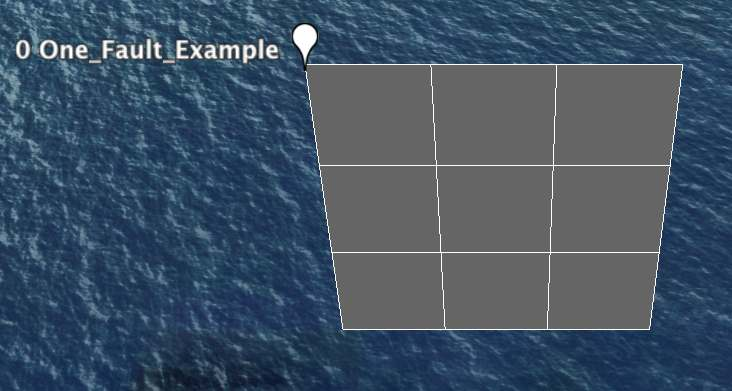
\includegraphics[height=5cm]{graphics/single_fault_4k}

}

\caption{\label{fig:meshing-example}A demonstration of meshing with different
resolutions.}
\end{figure}


Figure \ref{fig:meshing-example} shows the result of meshing the
One\_Fault\_Example trace with different element resolutions. Figures
\ref{fig:mesh6km} and \ref{fig:mesh4km} show the KML output of the
program in Google Earth (citation). Since the fault is defined to
start at latitude/longitude (0,0) it will appear in the middle of
the Atlantic ocean. In output KML files the depth is reversed so faults
are visible above the surface. When performing simulations with realistic
fault systems it is better to use actual fault latitude/longitude
in the traces to help visualize the simulation results.


\section{Element Stress Interactions}

Unlike actual fault systems where the fault geometry is dynamic over
long time periods, Virtual California simplifies calculations assuming
a geometrically static fault system. In this way Virtual California
is intended to explore seismicity in fault systems as they appear
today rather than attempting to model their long term evolution. Back
slip is used to model the effects of stress buildup and release along
elements approximating the fault plane. In a back slip model, the
equilibrium and initial positions of an element are the same, thus
when an element fails it moves towards the original position and the
fault system geometry remains static.


\subsection{Green's Functions}

Interactions between fault elements depend on the relative position
and orientation of each element, and are calculated using stress Green's
functions at the start of the simulation. The change in stress at
a location $x$ due to movement of all elements is given by \cite{Rundle2006vc}:

\begin{equation}
\sigma_{ij}(x,t)=\int dx_{k}^{'}T_{ij}^{kl}(x-x')s_{l}(x',t)\label{eq:stress_field}
\end{equation}


where $s_{l}(x',t)$ is the three-dimensional slip density of element
$l$, $T_{ij}^{kl}(x-x')$ is the Green's function tensor, and $l$
goes over all elements. In Virtual California this field is evaluated
only at the center of elements and slip is assumed to be uniform across
the surface of an element and along the element rake angle defined
in the model. Under these conditions equation \ref{eq:stress_field}
simplifies to:

\begin{equation}
\sigma_{ij}^{A}(t)=\sum T_{ij}^{AB}s_{B}(t)\label{eq:simple_stress_field}
\end{equation}


where B runs over all elements. Finally, since Virtual California
only uses the shear stress along the element rake vector and normal
stress perpendicular to the element, the tensor $T_{ij}^{AB}$ reduces
to $T_{s}$ for shear stresses and $T_{n}$ for normal stresses. This
means the shear and normal stresses on an element in Virtual California
are calculated as:

\begin{equation}
\sigma_{s}^{A}(t)=\sum T_{s}^{AB}s_{B}(t)\label{eq:shear_stress_sum}
\end{equation}


\begin{equation}
\sigma_{n}^{A}(t)=\sum T_{n}^{AB}s_{B}(t)\label{eq:norm_stress_sum}
\end{equation}


Thus, for a fault model with $N$ elements Virtual California requires
two $N\times N$ element matrices to represent all interactions. These
are also referred to as the Green's function matrices. The actual
values for the matrix entries are calculated using Okada's half-space
deformation equations \cite{Okada01041992}. Figure \vref{fig:okada_stress_field}
shows the stress field for a single vertical strike-slip fault element. 


\subsection{Event Transition Time}

Virtual California uses a combined static-dynamic friction law to
calculate element failures. This law is based on the Coulomb failure
function (CFF):

\begin{equation}
CFF^{A}(t)=\sigma_{s}^{A}(t)-\mu_{s}^{A}\sigma_{n}^{A}(t)\label{eq:cff_function}
\end{equation}


where $\mu_{s}^{A}$ is the static coefficient of friction on element
$A$ based on model element strengths. During long term stress accumulation,
an element is defined to fail at time $t_{f}$ when $CFF^{A}(t_{f})=0$,
which is referred to as static failure. At this point the simulation
changes to the rupture event model described below.

Given the change in stress over time it is relatively straightforward
to calculate the time to failure for an element. Since effective long
term slip rates during stress accumulation are assumed to be constant
the change in CFF over time is governed by the equation:

\begin{equation}
\frac{dCFF^{A}}{dt}=(\sigma_{s}^{A}-\mu_{s}^{A}\sigma_{n}^{A})+\alpha T_{\alpha}^{A}\label{eq:cff_change}
\end{equation}


where $\alpha$ represents the fraction of fault slip that is aseismic
and $T_{\alpha}^{A}=\frac{CFF^{A}T^{AA}}{rec}$ represents the instanteous
change in CFF due to aseismic slip. Aseismic slip on an element transmits
stress to other elements but not on the element itself. 

Knowing the relationship between slip and stress (equations \ref{eq:shear_stress_sum}
and \ref{eq:norm_stress_sum}), it is not necesary to evolve the system
time step by time step. Rather, the simulation time is advanced directly
to the point at which the next element fails. Equations \ref{eq:cff_function}
and \ref{eq:cff_change} allow us to analytically solve for the time
when the next element will fail.


\section{Rupture Event Model\label{sec:Event_Model}}

\begin{figure}[th]
\subfloat[CFF vs. time for a series of stress buildup and rupture events.]{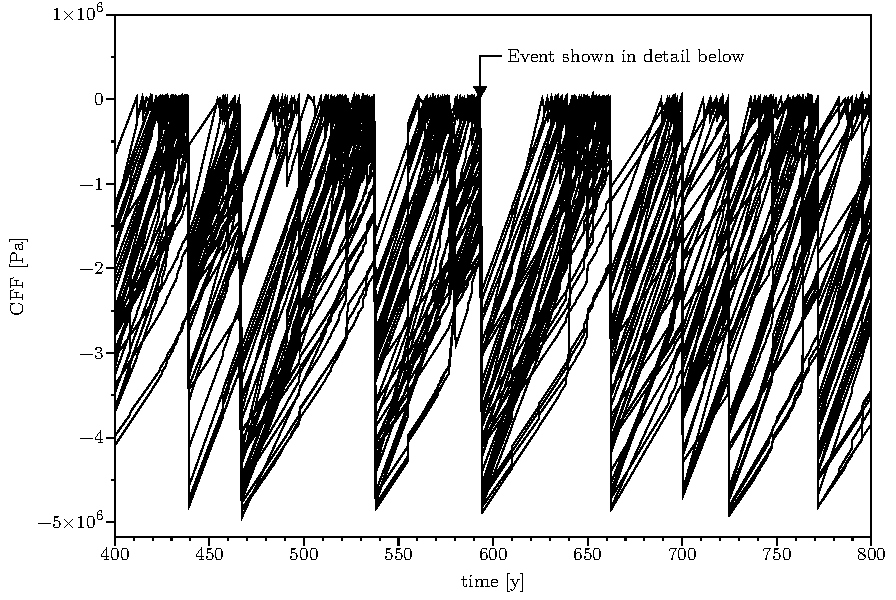
\includegraphics[width=0.48\textwidth]{graphics/CFF_1}

}\hfill{}\subfloat[CFF vs. sweeps for the event at t=593]{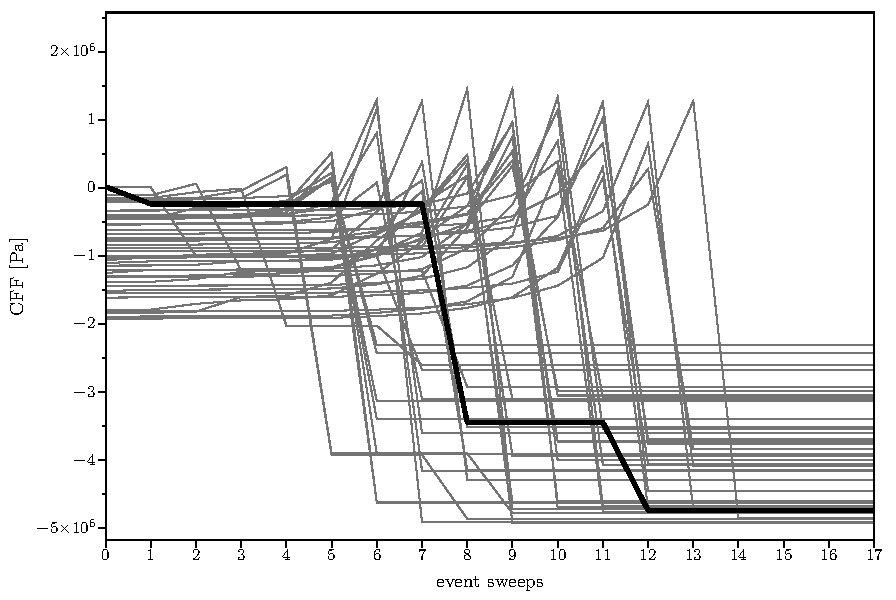
\includegraphics[width=0.48\textwidth]{graphics/CFF_2}

}\caption{Top: The CFF for each of the 48 elements comprising the Parkfield
section of the San Andreas fault. Drops in CFF correspond to stress
release in events, with larger events consisting of many elements
releasing stress. Bottom: detail of rupture sweeps from the event
at t=593. The trigger element is shown bold. Note that elements may
experience multiple failures, such as the trigger element failing
during sweeps 0, 7, and 11.\label{fig:cff_example_history}}
\end{figure}


During rupture propagation the first element to fail slips back towards
the equilibrium position. The amount of slip during the initial failure,
$\Delta s$, is related to the stress drop defined for the element
in the model, $\Delta\sigma$, by \cite{Rundle2006vc}:

\begin{eqnarray}
\Delta s & = & \frac{1}{K_{L}}\frac{N_{ef}}{S_{t}}(\Delta\sigma-CFF),\mbox{if }N_{ef}\leq S_{t}\label{eq:sst_one}
\end{eqnarray}


\begin{eqnarray}
\Delta s & = & \frac{1}{K_{L}}(\Delta\sigma-CFF),\mbox{otherwise}.\label{eq:sst_two}
\end{eqnarray}


where $K_{L}$ is the element's stiffness or self-stress defined as
$K_{L}=T_{s}^{AA}-\mu_{s}^{A}T_{n}^{AA}$. The factor $\frac{N_{ef}}{S_{t}}$
captures the current size of the rupture with $N_{ef}$ representing
the number of failed elements on the currently rupturing fault and
$S_{t}$ representing the slip-scaling threshold parameter. This factor
prevents small ruptures from excessively slipping.

Once the slip is calculated for one or more elements, a new stress
state for the entire system is calculated using Equations \ref{eq:shear_stress_sum}
and \ref{eq:norm_stress_sum}. Additional elements will fail if their
CFF = 0 (static failure). To better model rupture propagation dynamic
failure is also allowed during rupture events. Dynamic failure allows
elements on the same fault and physically nearby to failed elements
to themselves fail at a lower stress level than the static failure
criterion. This dynamic failure is based on the increase in stress
during the rupture event. An element experiences dynamic failure if
it is on the same fault as an already failed element and satisfies:

\begin{equation}
\frac{CFF_{init}-CFF_{final}}{CFF_{init}}>\eta\label{eq:dynamic_trigger}
\end{equation}


where $\eta$ is a user defined dynamic triggering parameter either
for the whole system or uniquely defined for each element. This parameter
approximates the stress intensity factor at the tip of a propagating
rupture.

During rupture propagation, elements that have not completely slipped
back to equilibrium may fail again (potentially multiple times) and
release more stress. However, elements may not slip away from equilibrium
meaning they cannot absorb stress released by other failed elements.
This reflects the fact that failed elements may not heal during a
rupture but also may not release all accumulated stress immediately.
It is also important to note that an element may not release all accumulated
stress during a rupture, due to the slip-scaling threshold (Equations
\ref{eq:sst_one} and \ref{eq:sst_two}) and dynamic triggering (Equation
\ref{eq:dynamic_trigger}), as well as the stress state of all elements
at the start of rupture. For example, if all elements are in a high
stress state then a small initial rupture can quickly propagate and
become a large stress release event, whereas if most elements are
in a low stress state then a large initial rupture may quickly stop
propagating and release relatively little stress.

Examples of stress accumulation and release over multiple phases of
long term stress accumulation and rupture events are shown in Figure
\ref{fig:cff_example_history}. The first figure shows how a single
element failure leads to a rupture spanning multiple elements and
how stress builds up and releases in cycles over time. The second
figure shows how elements may fail multiple times during different
sweeps in an event, but do not accumulate additional stress after
failing.


\section{Simulation Flow}

\begin{figure}[th]
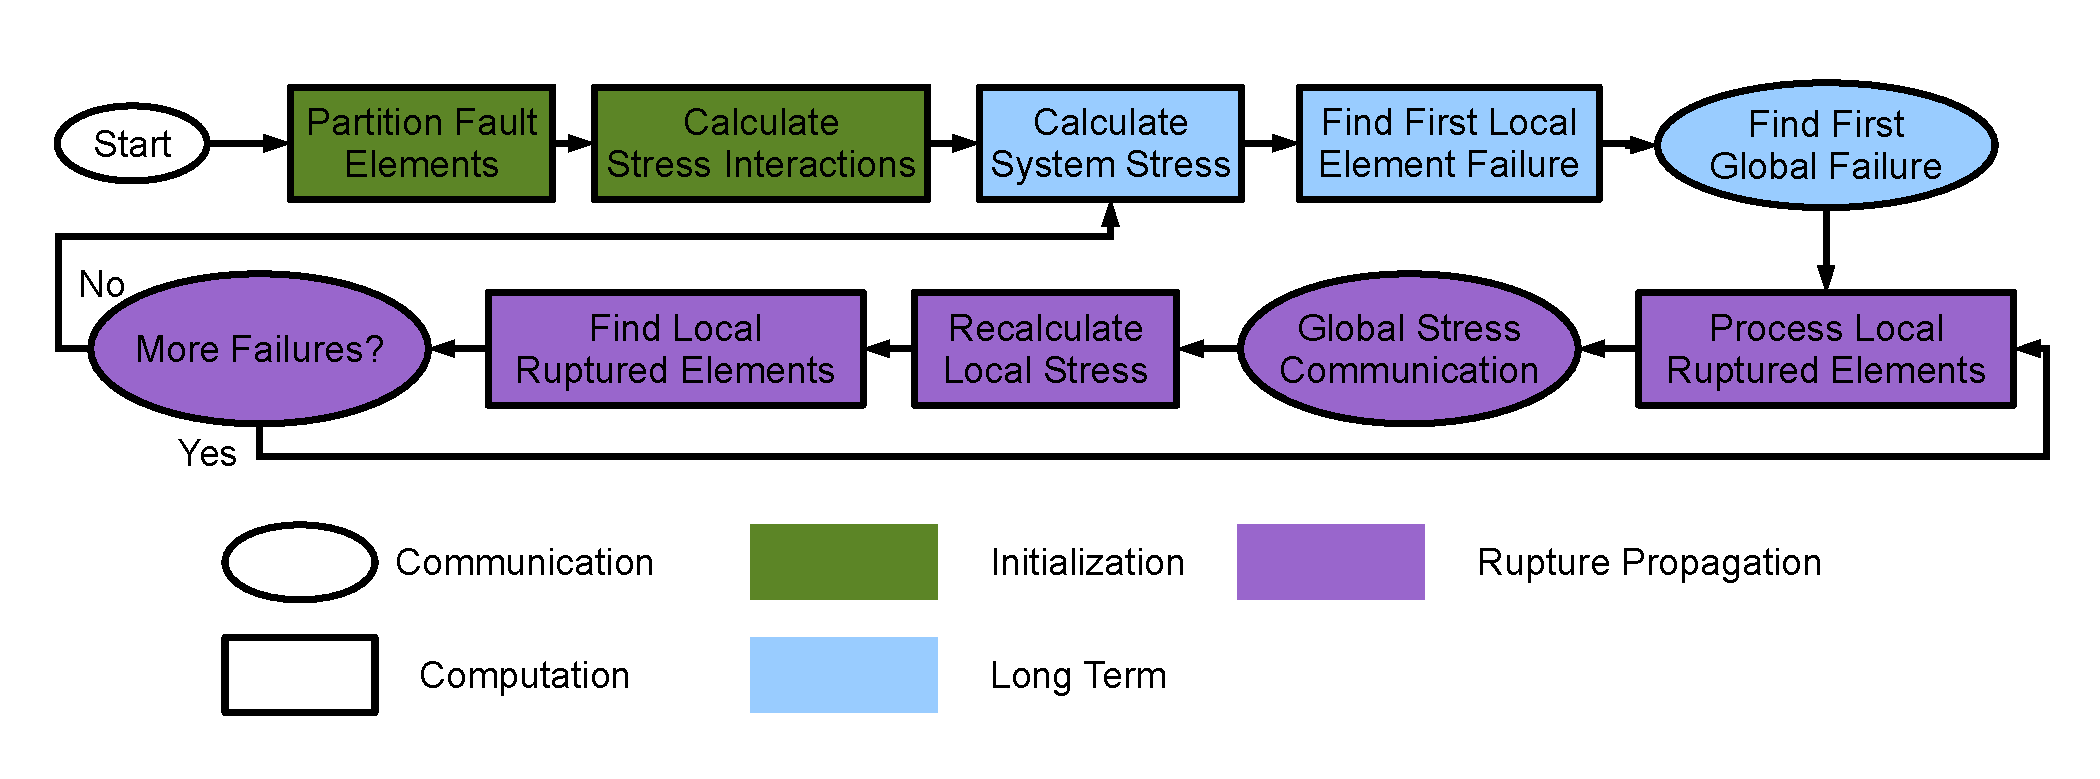
\includegraphics[width=0.99\textwidth]{graphics/VCFlow}\caption{Simulation flow of Virtual California.\label{fig:simulation_flow}}
\end{figure}
Figure \ref{fig:simulation_flow} shows the flow of simulation in
Virtual California. The simulation begins by reading in a set of faults
and converting them to the internal data structures. When running
a parallel simulation, these are partitioned over multiple processes
to ensure that each process is responsible for roughly an equal number
of elements and that elements on the same processor are on the same
fault or geographically close to each other. Next, each processor
calculates the stress Green's functions on the local elements for
all other elements in the model or loads precomputed Green's functions
from a file. This comprises the initialization phase of the simulation
shown in green in Figure \ref{fig:simulation_flow}.

The core of the simulation consists of repeated cycling between two
phases until the end of the simulation time. The first phase, shown
in blue, calculates the long term stress buildup and time to first
element failure in the system based on Equation \ref{eq:cff_function}.
In parallel simulations this time is calculated locally on each process
then reduced to a global time to failure.

The second phase is the rupture propagation phase, shown in purple
in Figure \ref{fig:simulation_flow}. Virtual California uses a cellular
automata style approach to modeling rupture propagation. The rupture
phase does not involve time domain solutions to differential equations,
but rather iterative calculations of stress and element failure to
approximate a rupture propagating through the fault system.


\section{QuakeLib Visual Tour}

As mentioned in Section \ref{sec:About_quakelib}, the QuakeLib library
provides tools and a Python interface to develop earthquake simulations,
read/write EqSim format files for geometry, friction, initial conditions
and events, and calculate Okada's functions for arbitrary fault geometries. 

QuakeLib can be compiled and used independently from Virtual California.
To only compile QuakeLib, follow the install instructions in section
\ref{sec:Install} but from the quakelib subdirectory.

This chapter provides a brief visual tour of a few analytical utilities
in QuakeLib and to illustrate its capacity as the computational backbone
for impressive and informative visualizations.


\subsection{Conventions}

The QuakeLib functions act on single fault elements, and compute various
dynamic quantities like the stress tensor, surface deformation field,
and gravity anomalies. These functions take fault parameter values
following Okada's convention \cite{Okada01041992}. Figure \ref{fig:okada_convention}
shows Okada's convention for fault plane elements in an elastic halfspace
$z \leq 0$. The two Lam� parameters ($\lambda$,$\mu$) that describe
the fault element's elasticity are also required. These parameters
and their units are described in detail in Appendix \ref{sec:Trace-File-Format}.

\begin{center}
\begin{figure}
\begin{centering}
\begin{minipage}[t]{0.45\columnwidth}%
\begin{center}
\subfloat{\noindent \centering{}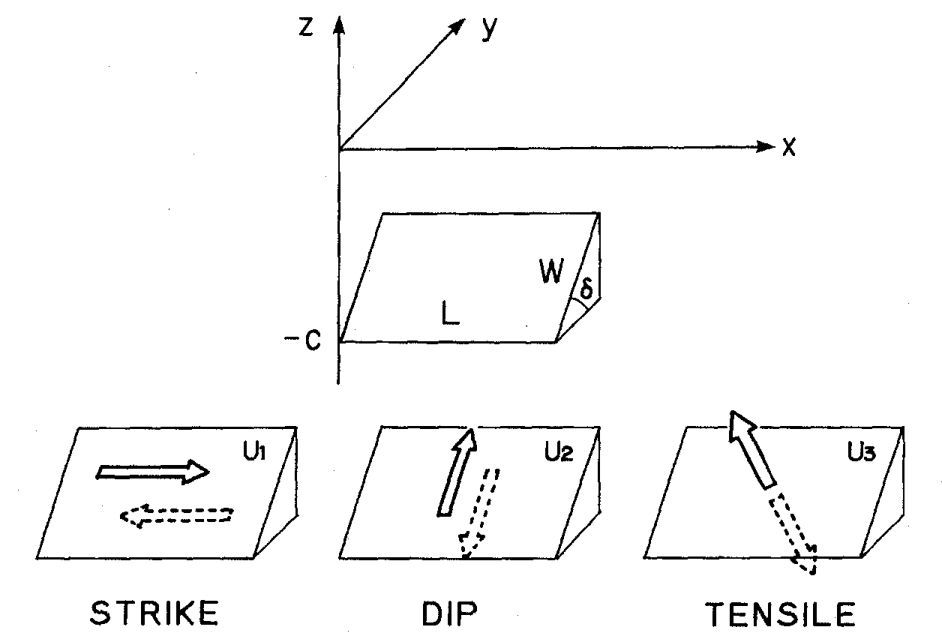
\includegraphics[bb=0bp 0bp 453bp 307bp,width=1\textwidth]{graphics/Okada_Fault_Convention}}
\par\end{center}%
\end{minipage}\hspace{1cm}%
\begin{minipage}[t]{0.35\columnwidth}%
\begin{center}
\subfloat{\raggedright{}%
\begin{tabular}{|c|c|}
\hline 
\textsf{\textbf{\small{Parameter}}} & \textsf{\textbf{\small{Description}}}\tabularnewline
\hline 
\hline 
\textsf{\small{L, W}} & \textsf{\small{Fault length, down-dip width}}\tabularnewline
\hline 
\textsf{\small{$\delta$}} & \textsf{\small{Dip angle}}\tabularnewline
\hline 
\textsf{\small{C}} & \textsf{\small{Fault plane depth}}\tabularnewline
\hline 
\textsf{\small{U1}} & \textsf{\small{Slip unit vector for strike-slip}}\tabularnewline
\hline 
\textsf{\small{U2}} & \textsf{\small{Slip unit vector for dip-slip}}\tabularnewline
 & \textsf{\small{(U2\textgreater{}0 thrust; U2\textless{}0 normal)}}\tabularnewline
\hline 
\textsf{\small{U3}} & \textsf{\small{Slip unit vector for tensile}}\tabularnewline
\hline 
\textsf{\small{z}} & \textsf{\small{Distance below surface}}\tabularnewline
\hline 
\textsf{\small{x/y}} & \textsf{\small{Distance on surface}}\tabularnewline
\hline 
\end{tabular}}
\par\end{center}%
\end{minipage}\hspace{1.5cm}
\par\end{centering}

\caption{QuakeLib defines each fault element with parameters following Okada's
convention.\label{fig:okada_convention}}
\end{figure}

\par\end{center}


\subsection{Single Element Examples}

The following example plots provide a brief window into QuakeLib's
analytical tools applied to single fault elements.


\subsubsection{Stress Field\label{sec:quakelib_stress_field}}

The stress field Green's function is defined in quakelib/src/QuakeLibOkada.cpp
as \textbf{calc\_stress\_tensor. }This function computes the stress
tensor at an arbitrary location = (x,y,z) around the fault plane.
Examples of the shear stress field -- equation \ref{eq:shear_stress_sum}
-- computed by QuakeLib for a single vertical ($\delta = 90^{\circ}$)
strike slip fault element are shown in Figure \ref{fig:okada_stress_field}.

\begin{center}
\begin{figure}
\begin{centering}
\subfloat[Front view]{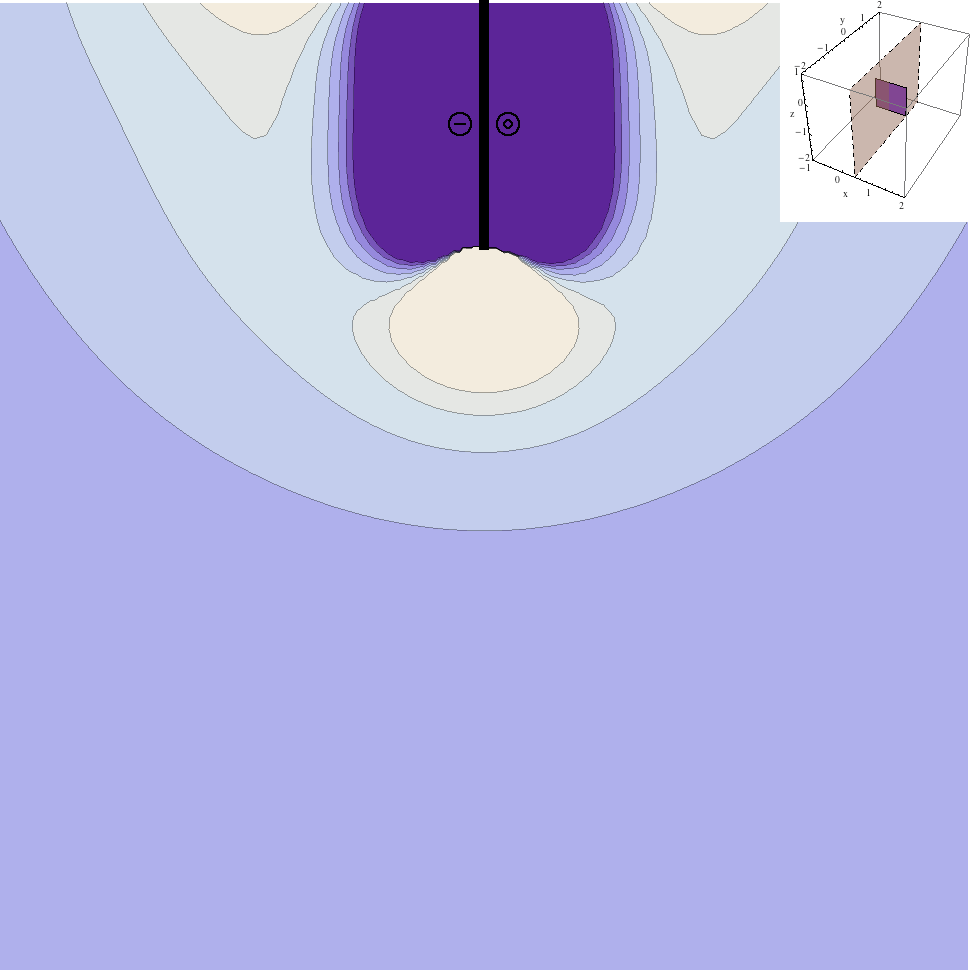
\includegraphics[width=0.42\textwidth]{graphics/sigma_s_front}

}\hfill{}\subfloat[Top view]{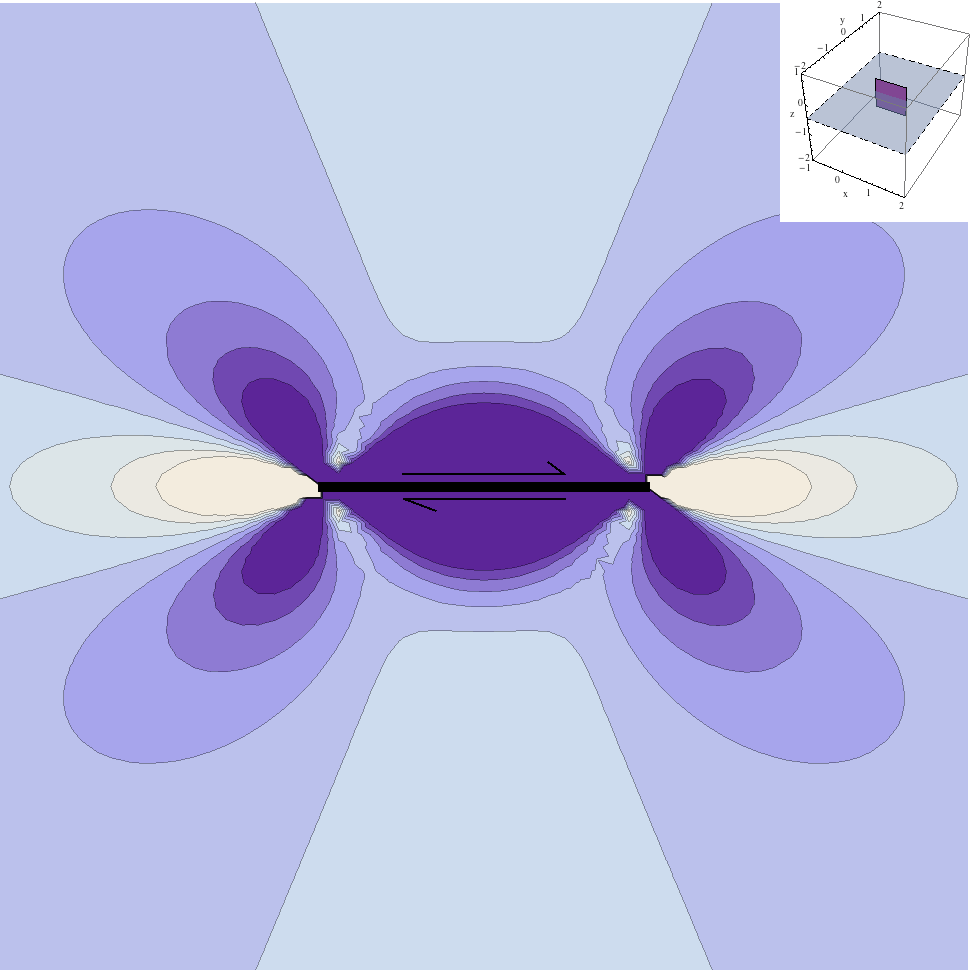
\includegraphics[width=0.42\textwidth]{graphics/sigma_s_top}}
\par\end{centering}

\caption{The shear stress field $\sigma_{xy}$ (tan $\sigma_{xy}>0$, blue
$\sigma_{xy}<0$) created by horizontal backslip, viewed from the
front and top of an element. The direction of backslip is indicated
by the arrows.\label{fig:okada_stress_field}}
\end{figure}

\par\end{center}


\subsubsection{Displacement Field}

The Green's function is defined in quakelib/src/QuakeLibOkada.cpp
as\textbf{ calc\_displacement\_vector.} This function computes the
co-seismic displacement vector for an arbitrary location = (x,y,z)
around the fault plane. The fault parameters for each fault element
are L = 10km, W = 10km, slip = 5m, and the horizontal/vertical axes
measure distance on the surface of the halfspace in km. The fault
plane depth values (C) are 10km for strike-slip, 11km for normal,
and 6km for thrust. The view is from above the fault plane looking
straight down at the surface, and the thick black lines are the projections
of the buried fault plane onto the surface of the halfspace.

\begin{center}
\begin{figure}
\begin{centering}
\begin{minipage}[t]{0.32\columnwidth}%
\begin{center}
\subfloat{\noindent \centering{}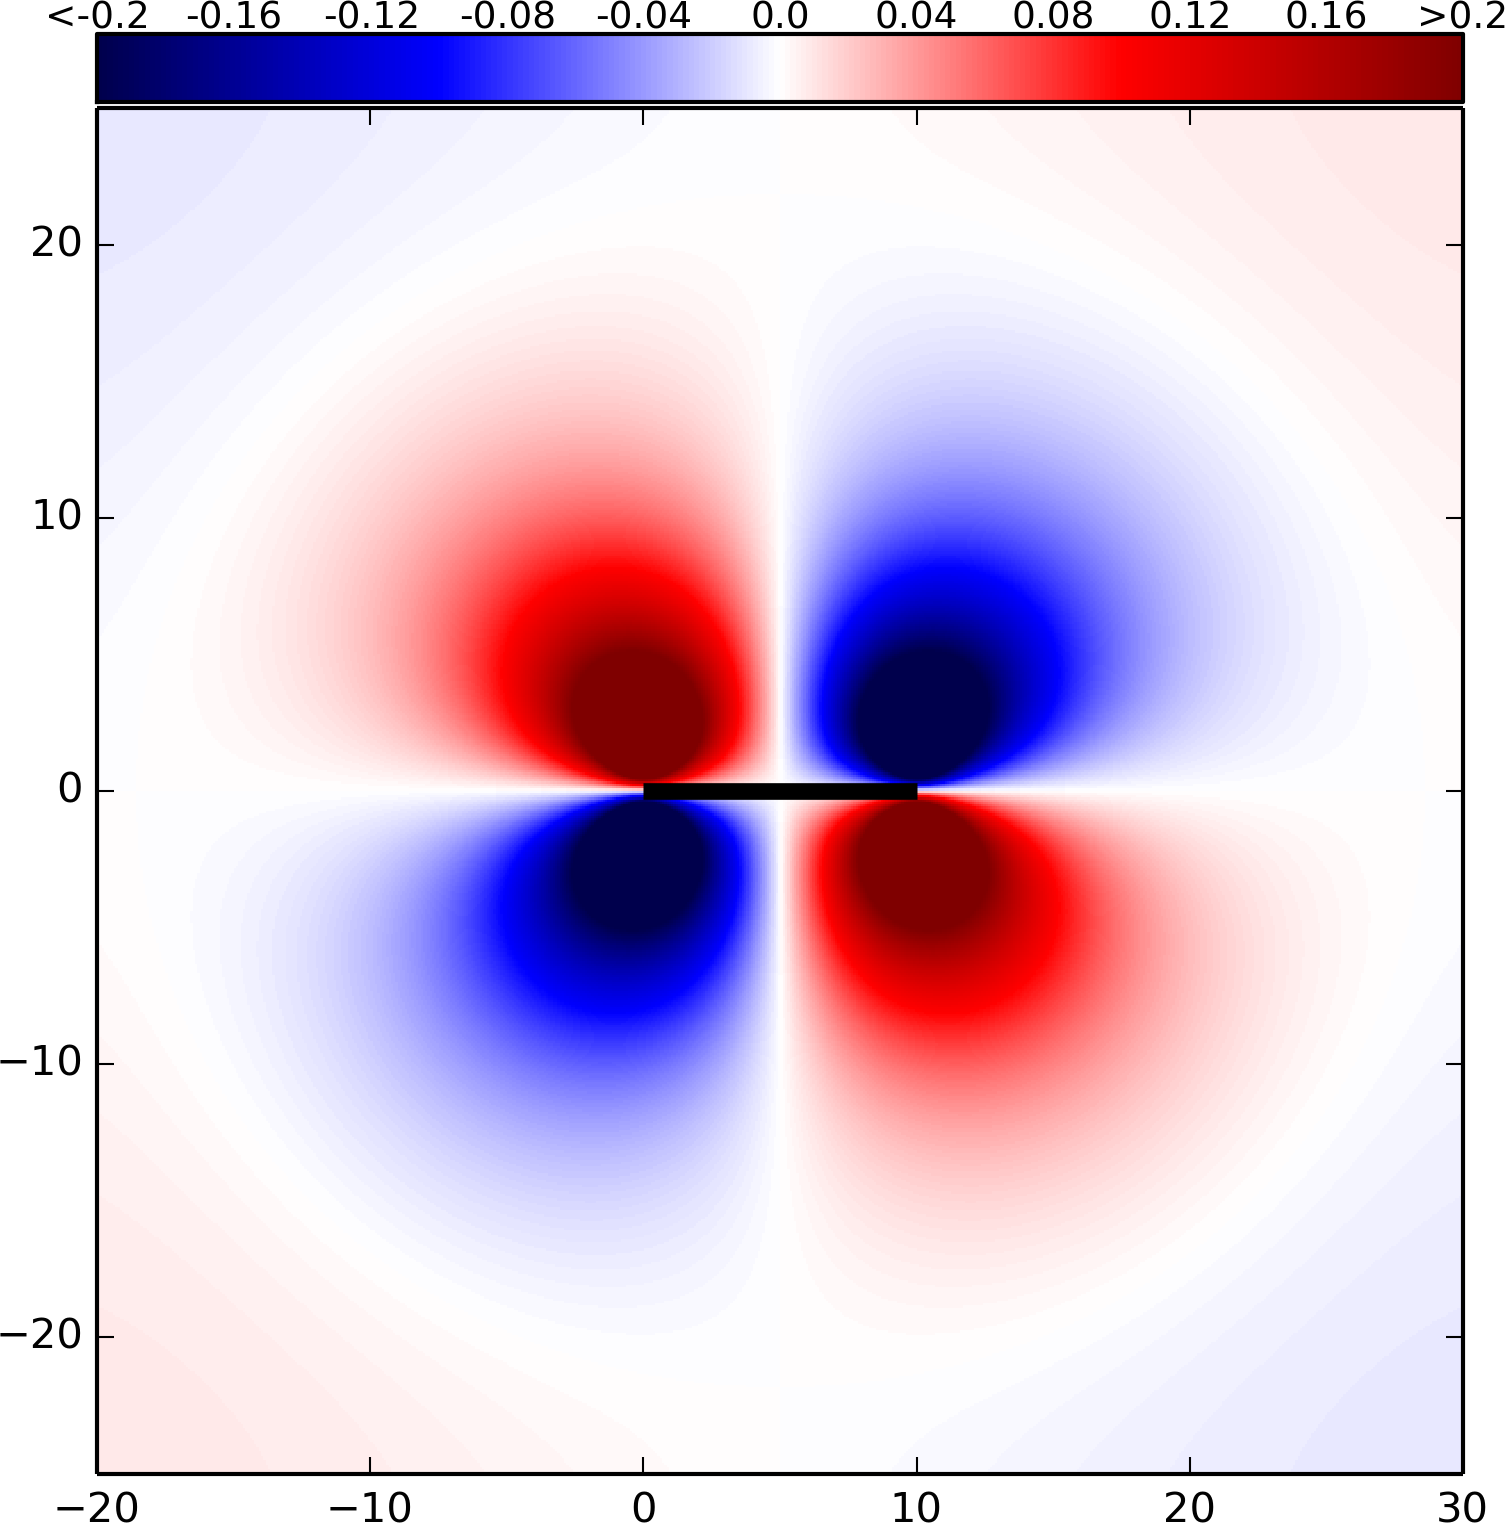
\includegraphics[width=1\textwidth]{graphics/dz_strikeslip5_dip90_L10k_W10k_c11k_docs_trim}}
\par\end{center}%
\end{minipage}\hfill{}%
\begin{minipage}[t]{0.32\columnwidth}%
\begin{center}
\subfloat{\noindent \centering{}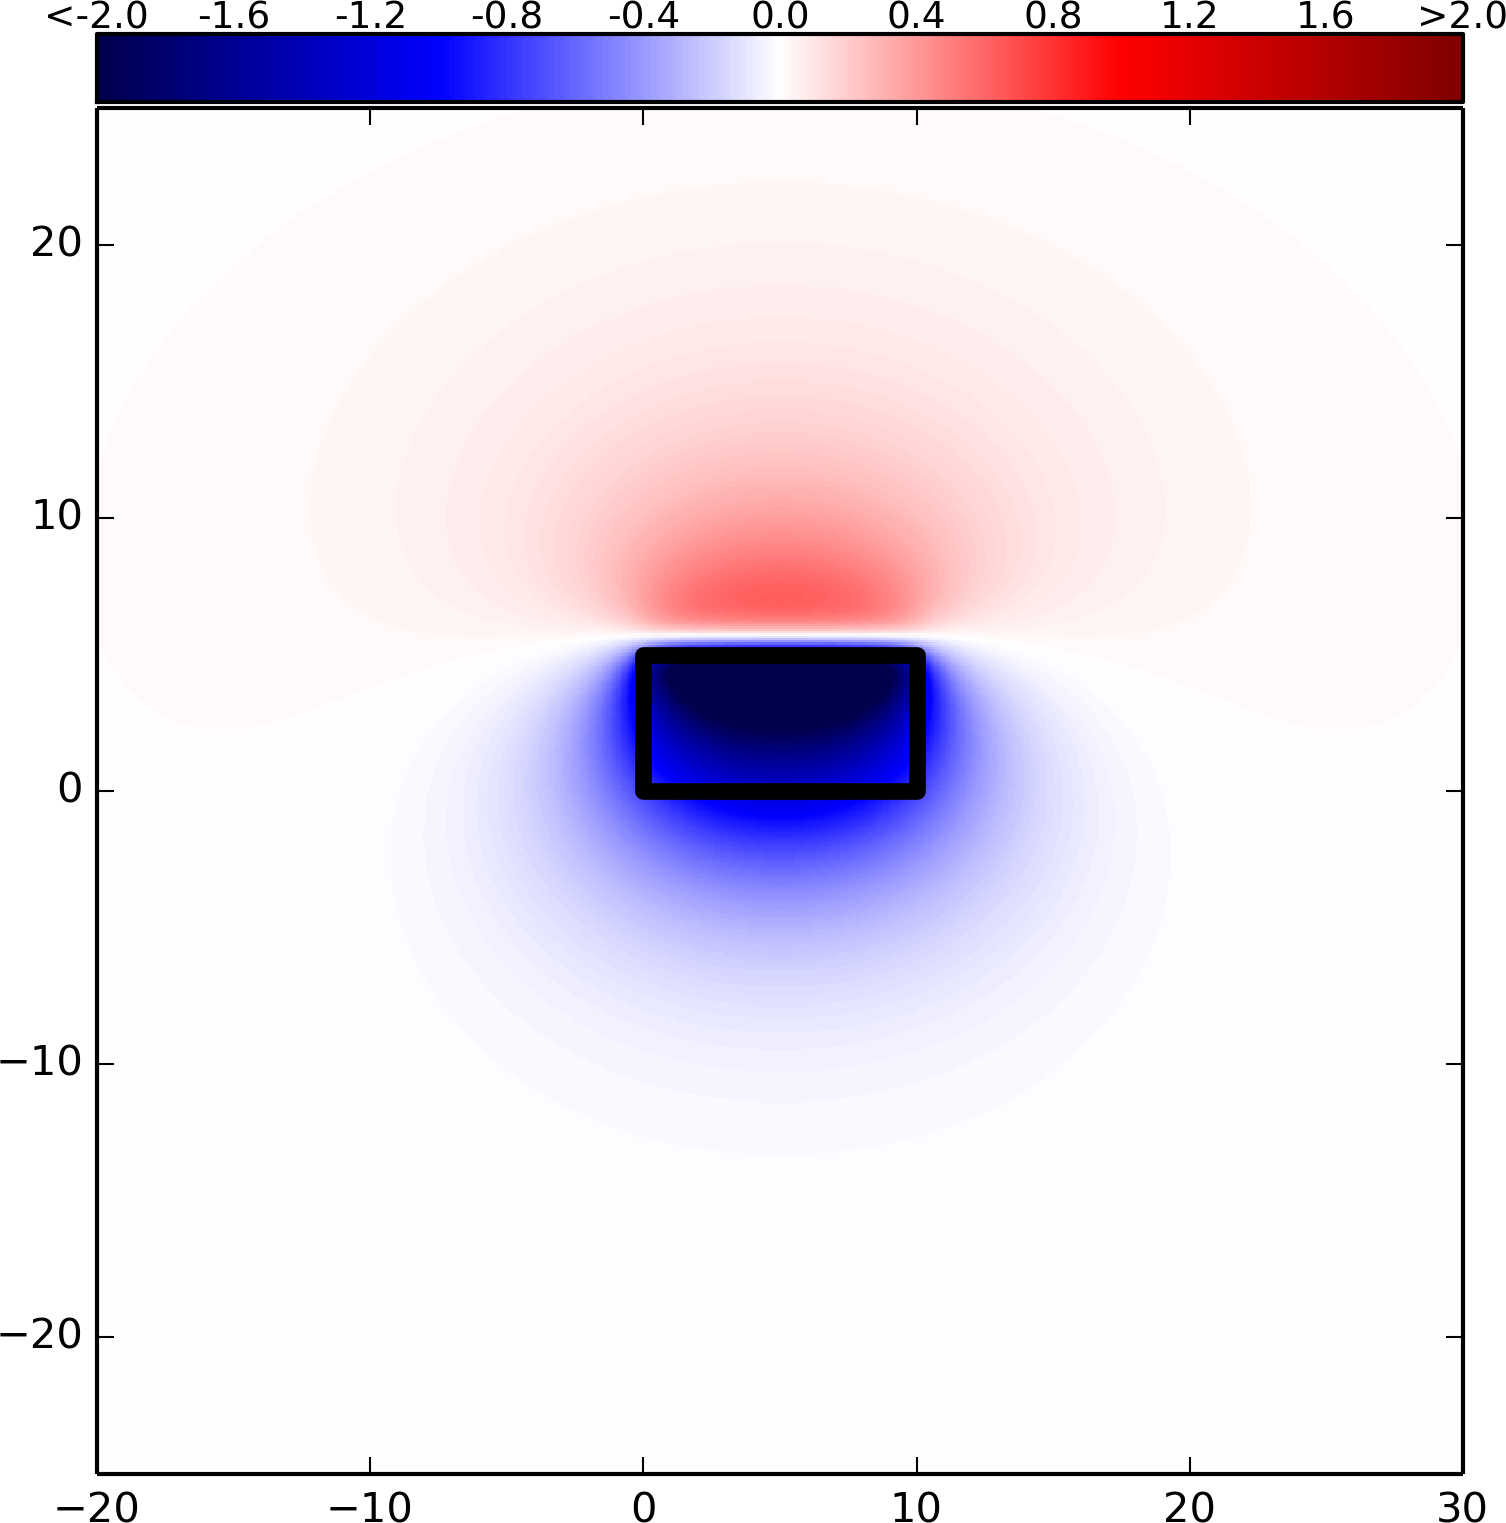
\includegraphics[width=1\textwidth]{graphics/dz_normal5_dip60_L10k_W10k_c10k_docs_trim}}
\par\end{center}%
\end{minipage}\hfill{}%
\begin{minipage}[t]{0.32\columnwidth}%
\begin{center}
\subfloat{\noindent \centering{}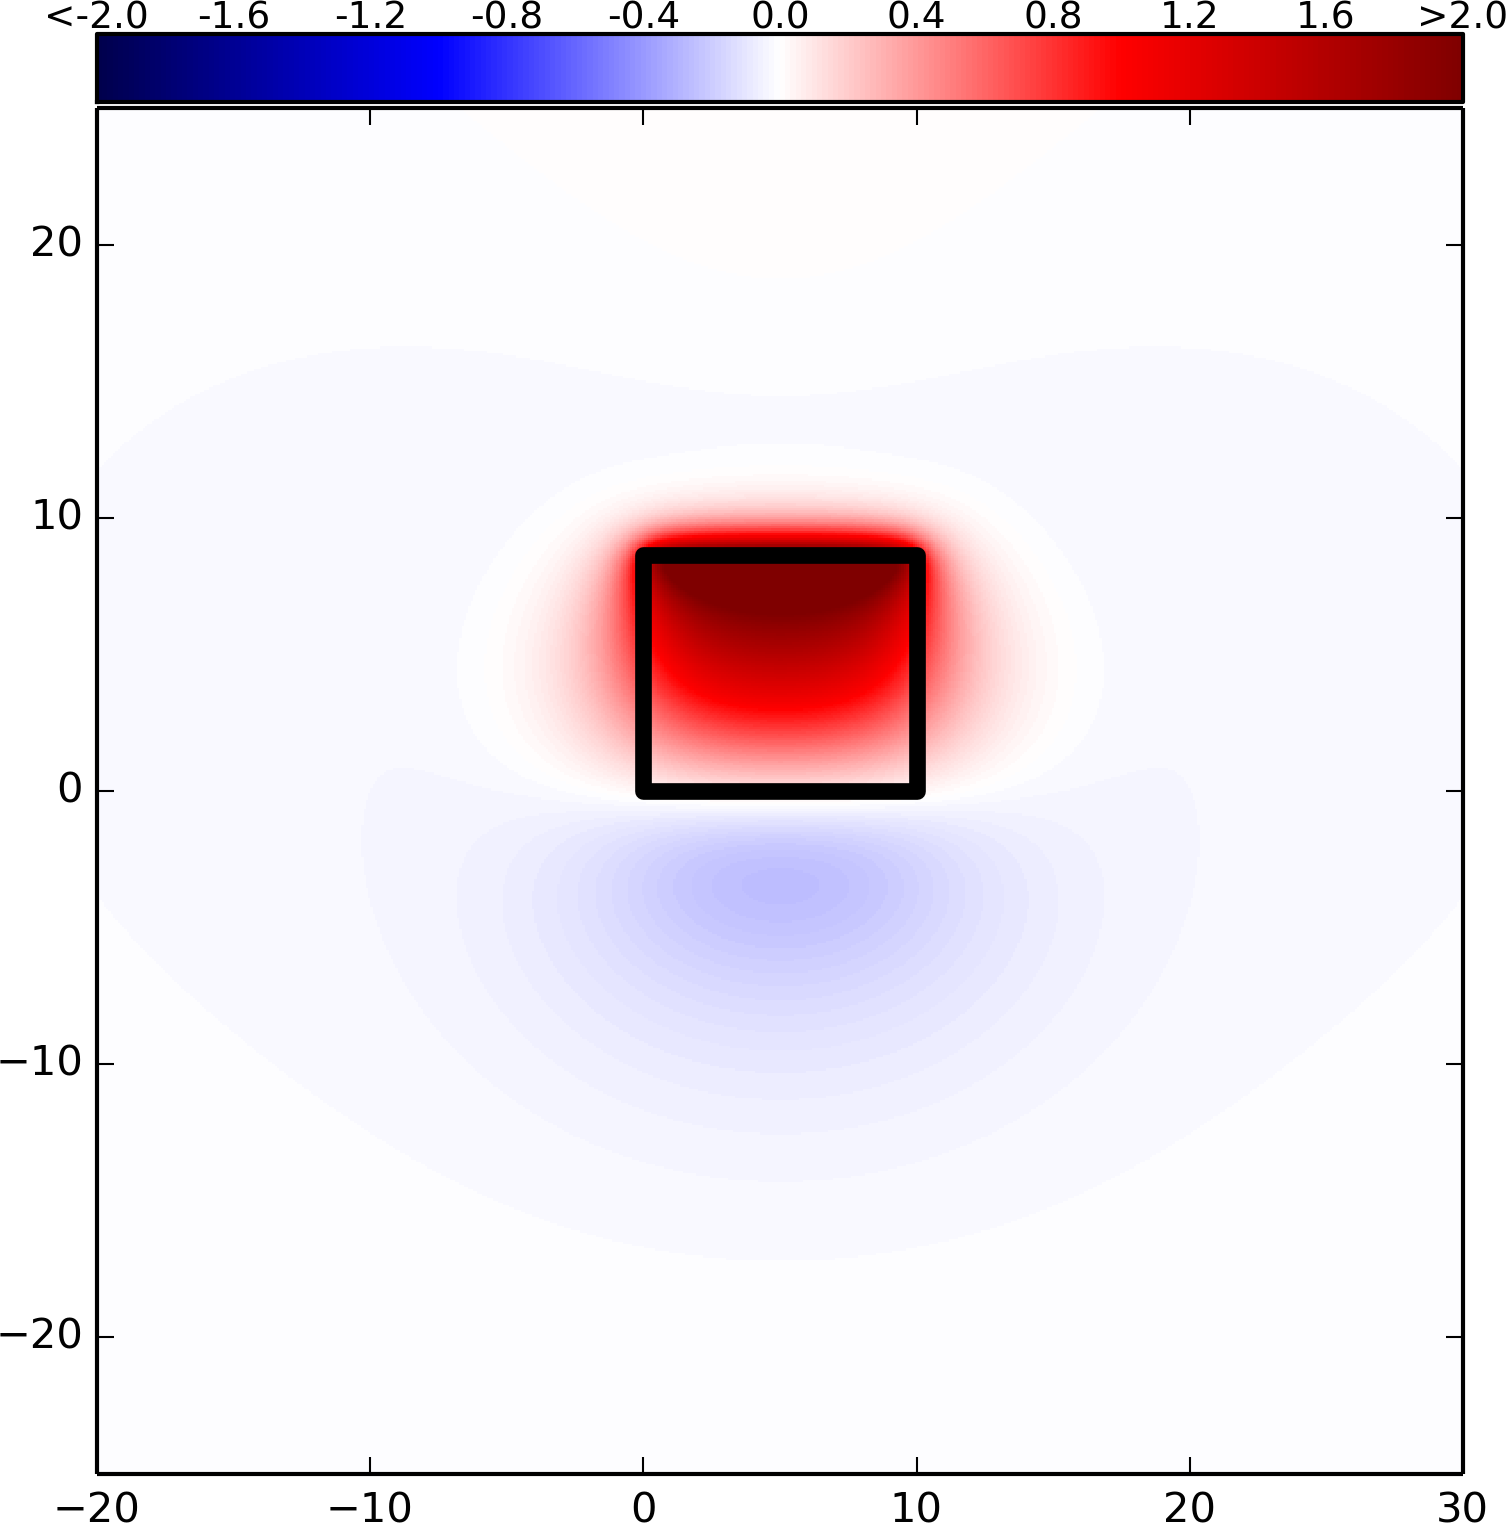
\includegraphics[width=1\textwidth]{graphics/dz_thrust5_dip30_L10k_W10k_c6k_docs_trim}}
\par\end{center}%
\end{minipage}
\par\end{centering}

\caption{Vertical displacement at the surface for buried fault elements, depth
to top of each fault plane is 1km, colorbar units are meters. \textbf{Left:}
strike-slip $\delta = 90^{\circ}$. \textbf{Center:} normal $\delta = 60^{\circ}$.
\textbf{Right:} thrust $\delta = 30^{\circ}$.\label{fig:single_element_displacements}}
\end{figure}

\par\end{center}


\subsubsection{Gravity Field Anomalies}

\begin{center}
The gravity Green's function is defined in quakelib/src/QuakeLibOkada.cpp
as \textbf{calc}\_\textbf{dg. }This function computes the gravity
anomalies at an arbitrary surface location = (x,y) around the fault
plane. This is the total gravity field anomaly Green's functions,
which includes contributions from subsurface density changes (dilatational)
and from surface displacement (free-air). Examples of the gravity
anomaly field for single fault elements is given in Figure \ref{fig:single_element_gravity_changes}.
The fault parameters are the same as above.
\par\end{center}

\begin{center}
\begin{figure}
\begin{minipage}[t]{0.32\columnwidth}%
\begin{center}
\subfloat{\noindent \centering{}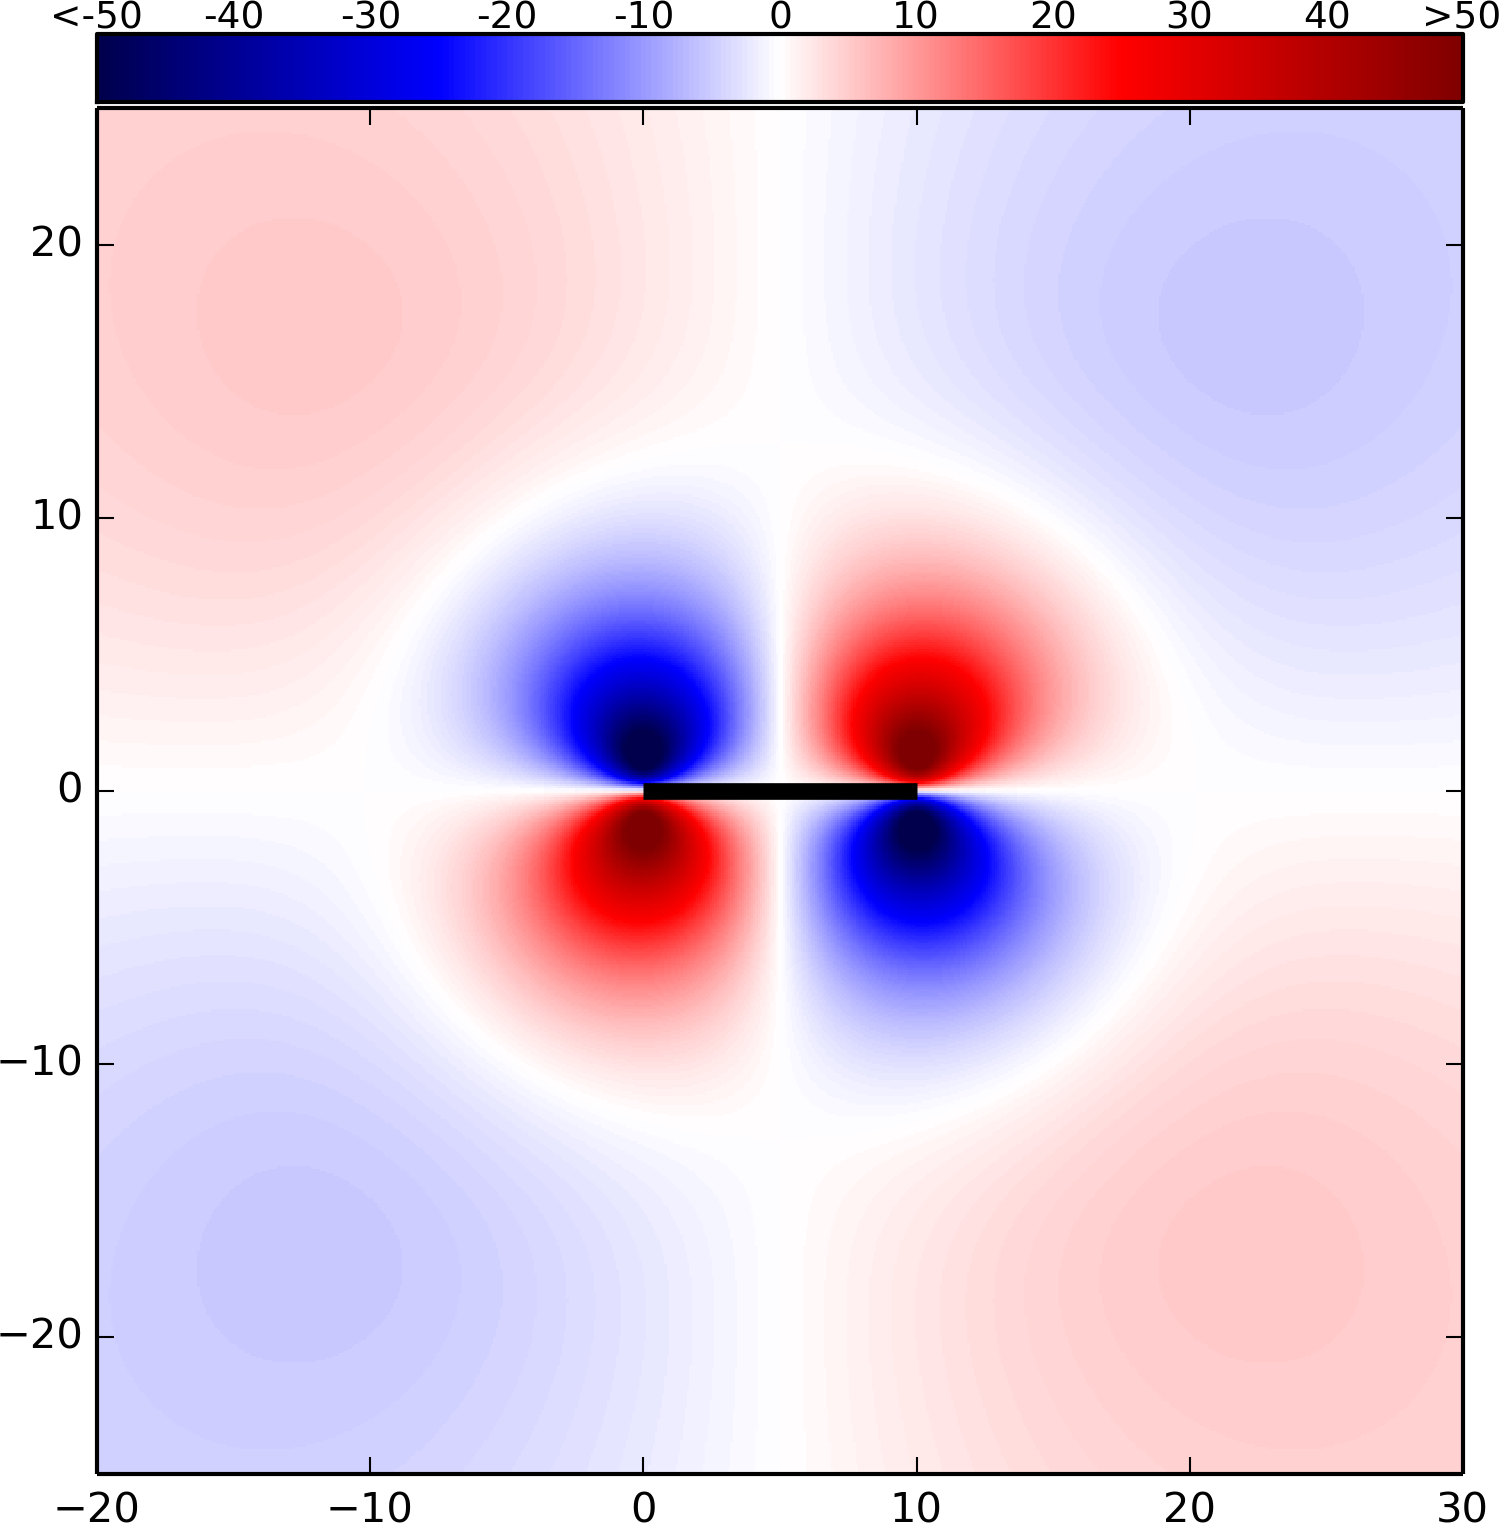
\includegraphics[width=1\textwidth]{graphics/dg_strikeslip5_dip90_L10k_W10k_c11k_docs_trim}}
\par\end{center}%
\end{minipage}\hfill{}%
\begin{minipage}[t]{0.32\columnwidth}%
\begin{center}
\subfloat{\noindent \centering{}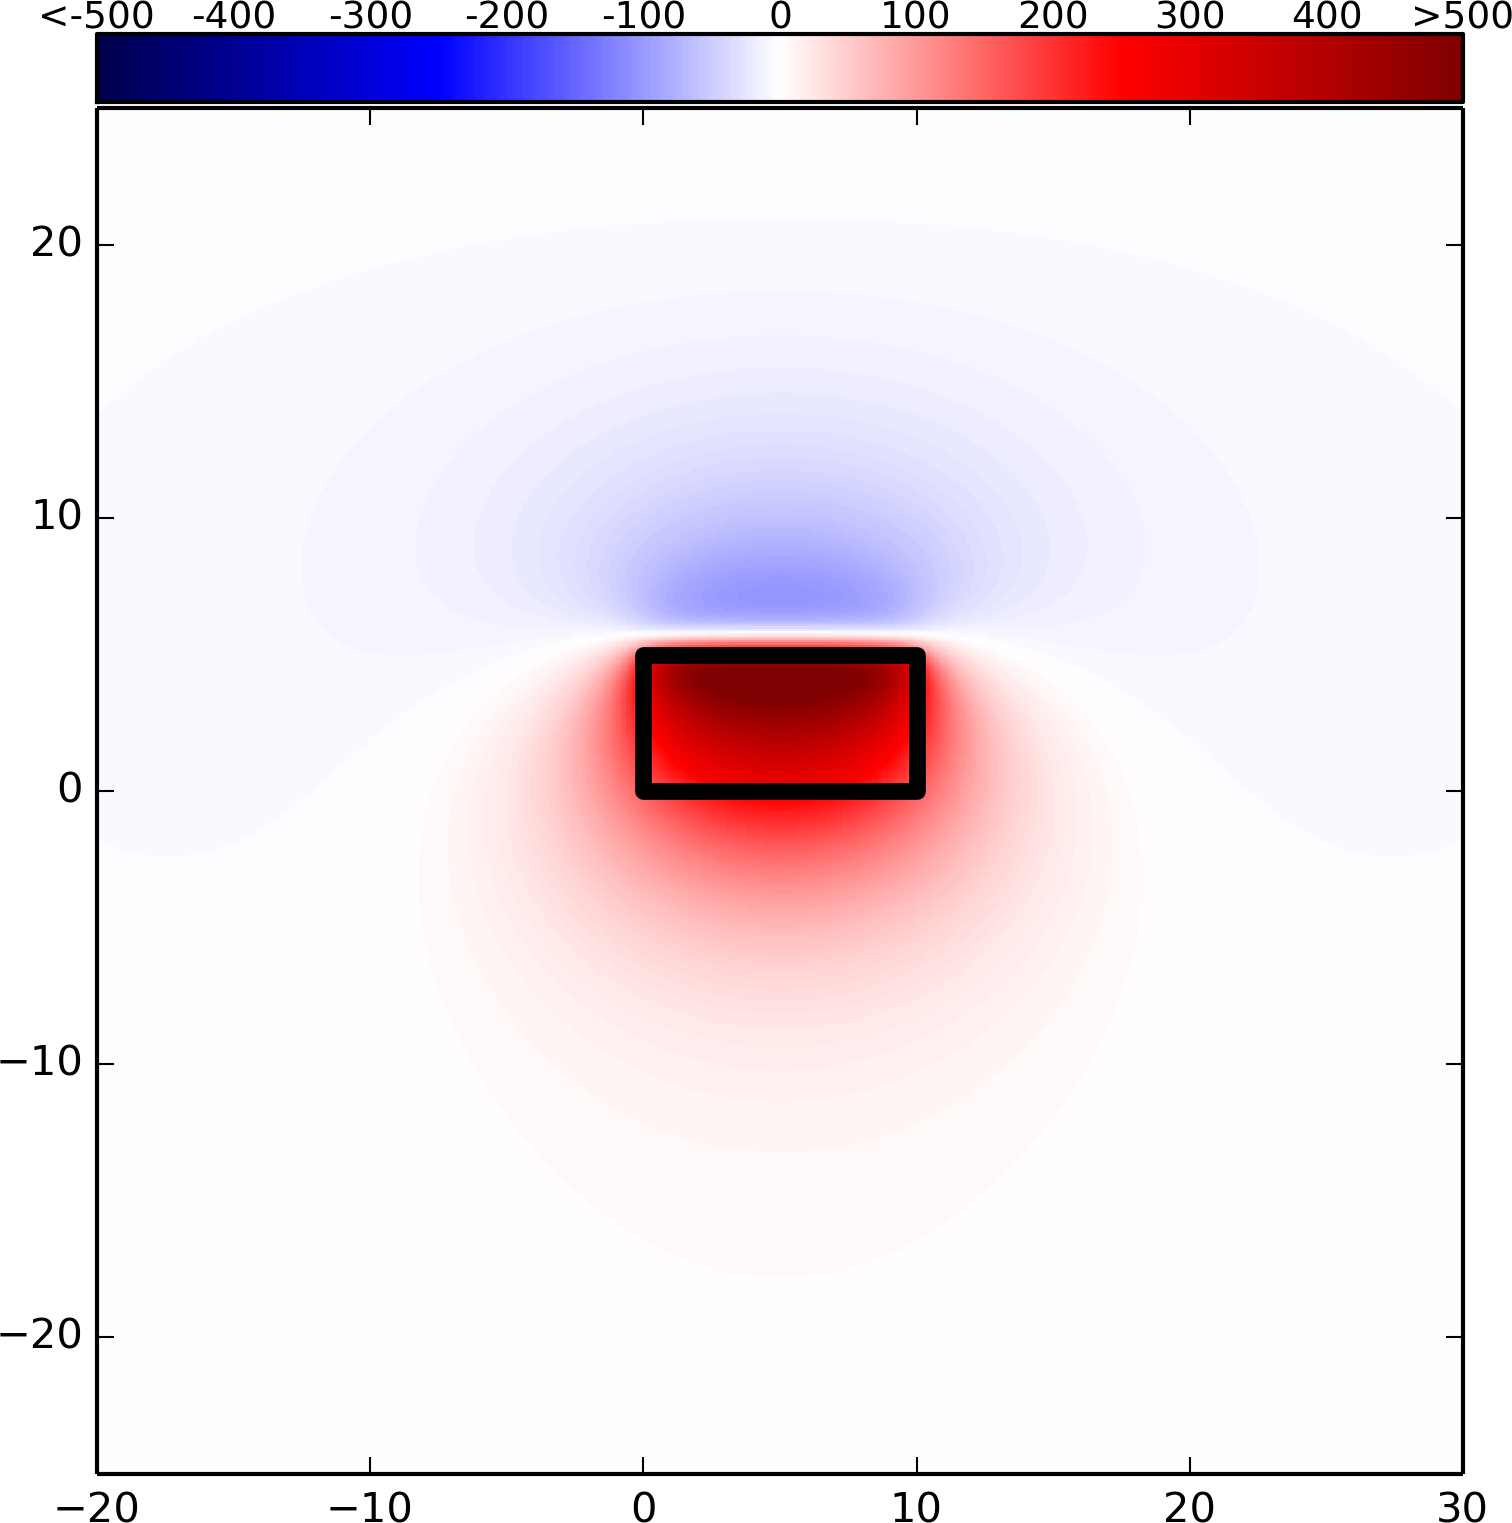
\includegraphics[width=1\textwidth]{graphics/dg_normal5_dip60_L10k_W10k_c10k_docs_trim}}
\par\end{center}%
\end{minipage}\hfill{}%
\begin{minipage}[t]{0.32\columnwidth}%
\begin{center}
\subfloat{\noindent \centering{}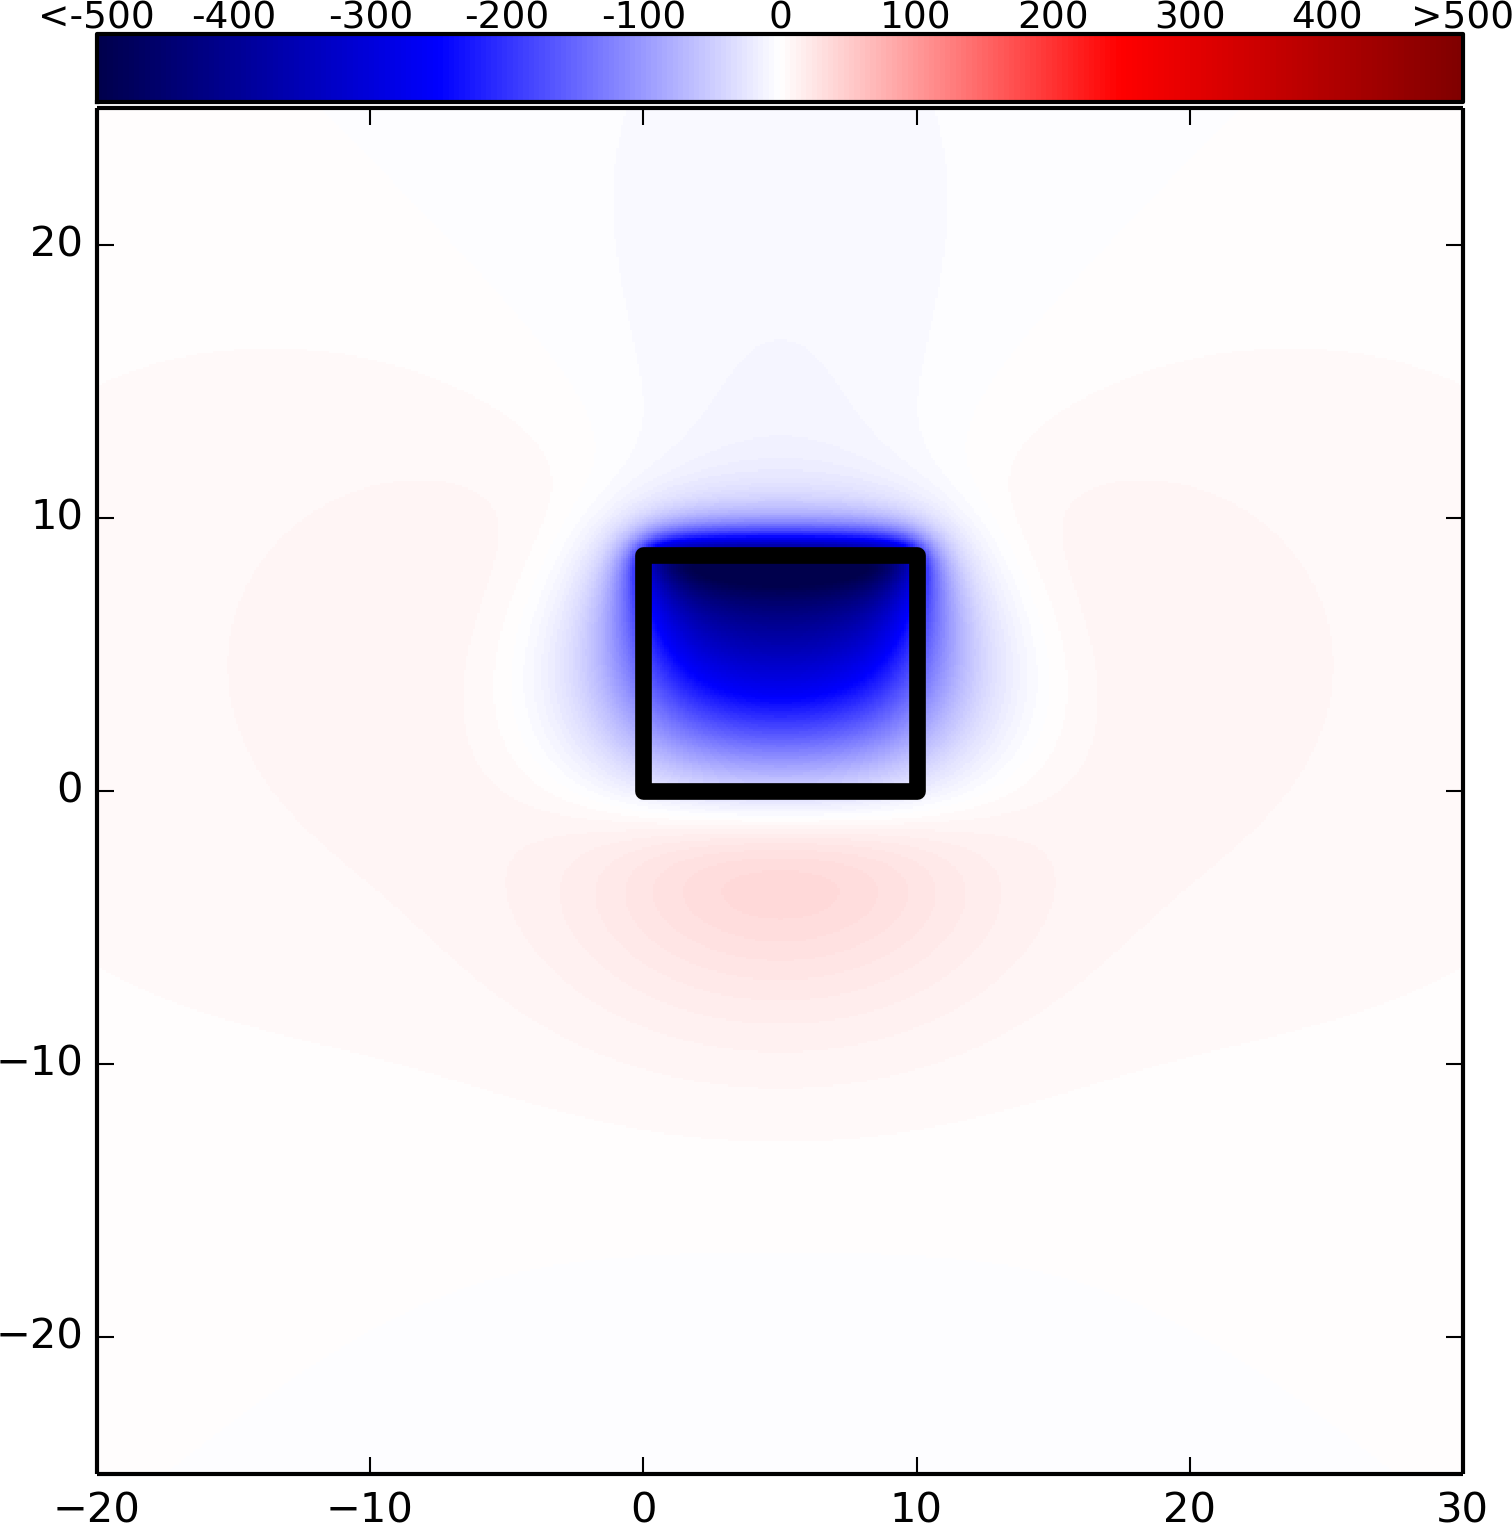
\includegraphics[width=1\textwidth]{graphics/dg_thrust5_dip30_L10k_W10k_c6k_docs_trim}}
\par\end{center}%
\end{minipage}

\caption{Gravitational anomalies for the fault elements in Figure \ref{fig:single_element_displacements},
colorbar units are $\mu gal$.\label{fig:single_element_gravity_changes}}
\end{figure}

\par\end{center}


\subsection{Topologically Realistic Examples}

The true power of QuakeLib lies in its ability to serve as the analytical
backbone for visualizing the results of Virtual California's simulated
seismic histories. The following example plots illustrate this point
by showing QuakeLib's tools applied over many fault elements involved
in a single simulated earthquake. The simulated earthquakes visualized
below come from a simulation involving all major fault sections in
California, the UCERF2 model described in section \ref{sec:Fault_model}.


\subsubsection{Displacement Field}

Figure \ref{fig:Displacement_field} shows vertical displacement field
on the surface as seen by an orbiting satellite for a very large (moment
magnitude 8.0) earthquake involving multiple sections of the San Andreas
Fault. 

\begin{figure}
\centering{}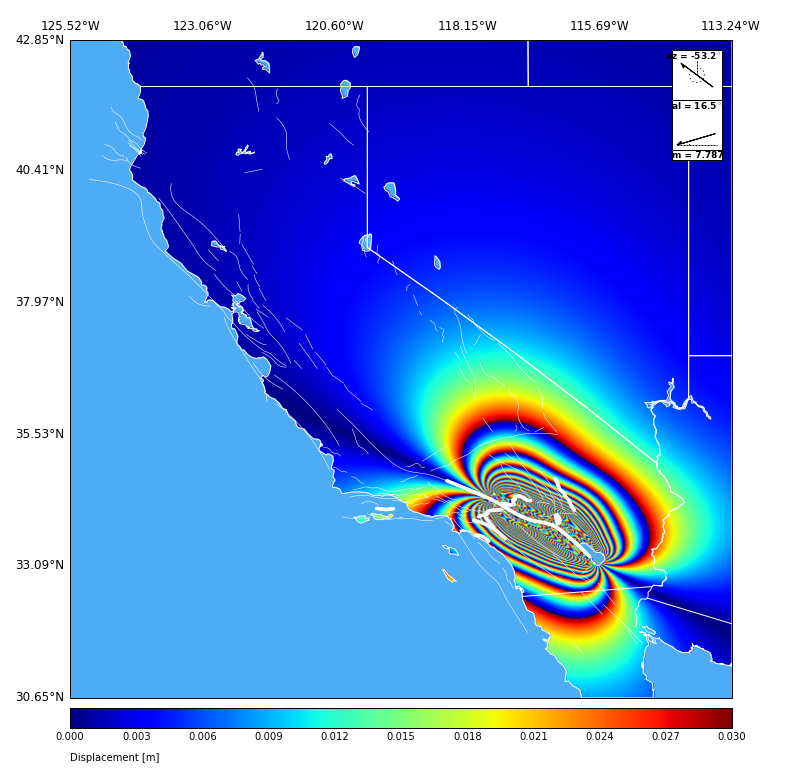
\includegraphics[width=1\textwidth]{graphics/dz_54358}\caption{\label{fig:Displacement_field}Simulated InSAR interferogram showing
vertical displacements for a large earthquake (moment magnitude 7.79)
involving multiple sections of the southern San Andreas Fault (thick
white lines), as seen by an orbiting satellite. }
\end{figure}



\subsubsection{Gravity Field Anomalies}

Figure \ref{fig:Gravity_field} shows co-seismic gravitational anomaly
field on the surface, possibly as measured by an orbiting satellite
for the same simulated earthquake as Figure \ref{fig:Displacement_field}. 

\begin{figure}
\centering{}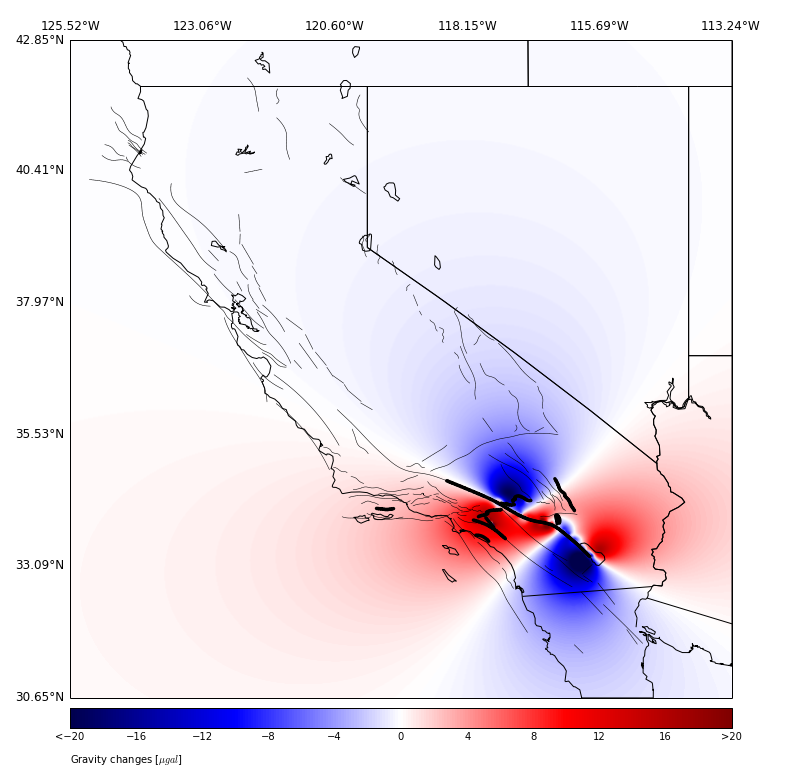
\includegraphics[bb=0bp 0bp 790bp 768bp,width=1\textwidth]{graphics/dg_54358}\caption{\label{fig:Gravity_field}Simulated surface gravity anomalies for
the same simulated earthquake as in Figure \ref{fig:Displacement_field}. }
\end{figure}



\chapter{Getting Started and Installation\label{cha:Installation}}


\section{Introduction}

Virtual California and QuakeLib have been tested on Linux, Mac OS
X and several other UNIX based platforms. Virtual California has also
been successfully run in parallel on several XSEDE systems and commodity
cluster systems. You should have no problems compiling, installing,
and running Virtual California on most Unix-like systems. Virtual
California is currently only available as a source package that users
must compile on their own. The following sections will lead you through
the installation process.


\section{Getting Help}

For help, send e-mail to the CIG Short Mailing List \url{cig-short@geodynamics.org}.
You can subscribe to the Mailing List and view archived discussion
at the Geodynamics Mail Lists web page \url{geodynamics.org/cig/lists}.


\section{System Requirements}

Installation of Virtual California requires a C++ compiler and the
headers and development libraries for
\begin{itemize}
\item MPI
\item OpenMP
\item HDF5
\item SWIG
\item CMAKE
\end{itemize}
You must also have Python 2.7 or greater installed.


\section{Downloading and Unpacking Source}

To obtain Virtual California, go to the Geodynamics Software Packages
web page \url{geodynamics.org/cig/software/vc}, download the source
archive and unpack it using the \texttt{tar} command: 
\begin{lyxcode}
\$~tar~xzf~VirtualCalifornia.tar.gz
\end{lyxcode}
If you don't have GNU Tar, try the following command instead: 
\begin{lyxcode}
\$~gunzip~-c~VirtualCalifornia.tar.gz~\textbar{}~tar~xf~-
\end{lyxcode}

\section{\label{sec:Install}Installation Procedure}

After unpacking the source, use the following procedure to install
the Virtual California executable as well as the QuakeLib library
and the mesher program:
\begin{enumerate}
\item Navigate (i.e., \texttt{cd}) to the directory containing the Virtual
California source\texttt{.}~\\
\texttt{}~\\
\texttt{\$ cd VirtualCalifornia}
\item Make the build directory\texttt{ and navigate to it.}~\\
\texttt{}~\\
\texttt{\$ mkdir build}~\\
\texttt{\$ cd build}
\item Use CMAKE to link everything before compiling VC.\texttt{}~\\
\texttt{}~\\
\texttt{\$ cmake ..}
\item Use CMAKE to build the package.\texttt{}~\\
\texttt{}~\\
\texttt{\$ make}
\end{enumerate}
If you are content to run Virtual California from the build directory,
then you are done. Upon successful completion, the \texttt{make} command
creates two executables ''mesher'' and \texttt{''vc''} in the
\texttt{/build/src/} subdirectory. VC is the script you will use to
run a Virtual California simulation, and the mesher program can create
fault models as described in section \ref{sec:building_faults}. You
may wish to add the \texttt{bin} directory to your \texttt{PATH}.

For more details about \texttt{configure}, see Section \ref{sec:Configuration}
below.


\subsection{Mac OS X}

With the OS X default python: 
\begin{lyxcode}
\$~mkdir~build

\$~cd~build

\$~cmake~..

\$~make
\end{lyxcode}
If you have a third party installation of python (ie. from homebrew
or macports) Virtual California will build and install, but the python
quakelib module may not work. This is because cmake builds against
the system python. To fix this do the following: 
\begin{lyxcode}
\$~./configure
\end{lyxcode}
cmake will output the following: 
\begin{lyxcode}
-{}-~Found~PythonLibs:~/usr/lib/libpythonx.x.dylib~
\end{lyxcode}
where \char`\"{}x.x\char`\"{} is a version number (ie. \char`\"{}2.7\char`\"{}).
We need to move this file and create a link to the correct python. 
\begin{lyxcode}
\$~sudo~mv~/usr/lib/libpythonx.x.dylib~/usr/lib/libpythonx.x.sys.dylib~

\$~which~python~\textbar{}~xargs~otool~-L~
\end{lyxcode}
This will output /the/path/to/python/library. 
\begin{lyxcode}
\$~sudo~ln~-s~/the/path/to/python/library~/usr/lib/libpythonx.x.dylib

\$~rm~-r~build/~

\$~./configure~

\$~cd~build~

\$~make~

\$~sudo~make~install~
\end{lyxcode}

\subsection{Linux}

Follow the steps below:
\begin{lyxcode}
\$~mkdir~build

\$~cd~build

\$~cmake~..

\$~make
\end{lyxcode}

\subsection{Install Locations}

Quakelib libraries will be installed in standard library directories
based on your system configuration. Cmake will generate a file named
\char`\"{}install\_manifest.txt\char`\"{} in the build directory detailing
the locations of installed files. The Virtual California binary is
build/src/vc.


\subsection{Selecting a Compiler}

Depending on the machine used to run VC, you may need to change which
compiler CMake uses to compile VC. For example, if the user wants
to compile VC with gcc 3.3, execute cmake as shown below.
\begin{lyxcode}
\$~CC=gcc-3.3~CXX=g++-3.3~cmake~..
\end{lyxcode}

\subsection{Additional Tools}

While the following software is not necessary for the normal operation
of Virtual California, you may find it useful for accessing Virtual
California data in HDF5 files.


\subsubsection{NumPy}

NumPy is an extension to Python which adds support for multi-dimensional
arrays for use in scientific computing. You may download NumPy from
the NumPy home page \url{numpy.scipy.org}. To compile and install
this extension, download it and issue the following commands after
extracting it:
\begin{lyxcode}
\$~cd~numpy-1.0

\$~python~setup.py~install~-{}-prefix=\$HOME/cig
\end{lyxcode}
Alternatively, under Debian Linux you can install the \texttt{python-numpy}
package. On Gentoo Linux, NumPy is available in the \texttt{dev-python/numpy}
ebuild.


\subsubsection{PyTables}

PyTables is a package for managing hierarchical datasets and designed
to efficiently and easily cope with extremely large amounts of data.
PyTables is built on top of the HDF5 library, using the Python language
and the NumPy package. After checking its dependencies, you may download
PyTables from the PyTables home page \url{pytables.org}. To install,
follow instructions on the installation page \url{http://pytables.github.io/usersguide/installation.html}. 


\subsubsection{HDFView}

HDFView is a visual tool written in Java for browsing and editing
HDF5 files. You may download it from the HDFView home page \url{hdf.ncsa.uiuc.edu/hdf-java-html/hdfview}.


\chapter{Running VC\label{cha:Running_VC}}


\section{Introduction}

Now that installation and testing is finished, let's get into the
specifics of building a fault model, compiling Virtual California,
and finally running a custom simulation. The following chapter serves
to illustrate the main features of a Virtual California simulation,
and will prepare the user for the explicit examples in Chapter \ref{cha:Running_VC}. 


\section{Basic Usage and Tests}

The main procedure for running a VC simulation is to create/assimilate
the fault model and friction parameters into a folder (see sections
\ref{sec:Tutorial_single} and \ref{sec:Tutorial_multiple} for examples),
compile Virtual California following Section \ref{sec:Install} to
generate the executable, place the executable in the same folder as
the parameter files, and finally execute the program. 


\subsection{CMake Tests}

If you installed Virtual California according to Section \ref{sec:Install},
then you successfully compiled the QuakeLib library and the VC and
mesher executables. We used CMake to compile the simulation program,
and we have also configured CMake to run a suite of unit tests and
even test simulations. To run the suite of unit tests simply type
the following into your terminal.
\begin{lyxcode}
\$~cd~VirtualCalifornia/build/

\$~make~test

Running~tests...~

Test~project~/Users/{[}username{]}/vc/build~

~~Start~1:~CondUnitTest~

1/79~Test~\#1:~CondUnitTest~.........................~Passed~0.11~sec~

~~Start~2:~FricUnitTest~

2/79~Test~\#2:~FricUnitTest~.........................~Passed~0.03~sec~

~~Start~3:~GreenUnitTest~

3/79~Test~\#3:~GreenUnitTest~........................~Passed~0.08~sec~

~~Start~4:~OctreeTest~

4/79~Test~\#4:~OctreeTest~...........................~Passed~0.13~sec~

~~Start~5:~UtilUnitTest~

5/79~Test~\#5:~UtilUnitTest~.........................~Passed~0.15~sec~

~~Start~6:~EventUnitTest~

6/79~Test~\#6:~EventUnitTest~........................~Passed~0.01~sec~

~~Start~7:~GeomUnitTest~

7/79~Test~\#7:~GeomUnitTest~.........................~Passed~0.04~sec~

~~Start~8:~MetadataUnitTest~

8/79~Test~\#8:~MetadataUnitTest~.....................~Passed~0.11~sec~

~~Start~9:~RectBoundTest~

9/79~Test~\#9:~RectBoundTest~........................~Passed~0.00~sec~

~~Start~10:~mesh\_single\_12000~

10/79~Test~\#10:~mesh\_single\_12000~....................~Passed~0.02~sec~

~~Start~11:~run\_single\_12000~

11/79~Test~\#11:~run\_single\_12000~.....................~Passed~0.16~sec~

~~Start~12:~test\_consistent\_single\_12000~

12/79~Test~\#12:~test\_consistent\_single\_12000~.........~Passed~0.06~sec~

~~Start~13:~test\_slip\_single\_12000~

13/79~Test~\#13:~test\_slip\_single\_12000~...............~Passed~0.03~sec

...

79/79~Test~\#79:~test\_consistent\_taper\_renorm\_2000~....~Passed~0.39~sec



100\%~tests~passed,~0~tests~failed~out~of~79

Total~Test~time~(real)~=~~~5.51~sec
\end{lyxcode}
The example output from the CMake test suite shows the range of output,
however you should not see any failed tests. The final lines of the
output summarize the results from the unit tests and test simulations. 


\subsection{Explicit Test Simulation\label{sec:Single-Processor-Test}}

If you would rather explicitly follow the steps of building your own
fault model, generating the parameter files and running the simulation,
then you should consult the tutorial in section \ref{sec:Tutorial_single}. 


\section{Advanced Usage}

Since the simulation physics and event model will work with any arbitrarily
complex fault model, advanced users can make Virtual California generate
simulated seismic histories for any fault system. The only requirement
for using VC to simulate dynamics on an arbitrary fault network is
to prepare the input files. Chapter \ref{cha:Running_VC} contains
examples that illustrate this procedure of defining fault geometry
and properties.


\subsection{Tuning Parameters\label{sec:tuning_parameters}}

Fault simulations must initially be tuned to correctly simulate actual
earthquakes. The primary tuning parameters in Virtual California are
the dynamic triggering factor $\eta$ and slip scaling threshold $S_t$,
defined in Section \ref{sec:Event_Model}. The dynamic triggering
factor is used to encourage rupture propagation during a simulated
earthquake. The slip scaling parameter is used to prevent small ruptures
from slipping too much. These parameters act to tune the rupture and
slipping properties of faults without requiring field measurements
of each fault's physical properties, a result of VC's abstraction
and generality. Currently, these parameters are set globally for the
fault model. Figure \ref{fig:tuning_parameters} shows a comparison
of simulation results for a range of these parameter values.

\begin{center}
\begin{figure}
\begin{minipage}[t]{0.48\columnwidth}%
\begin{center}
\subfloat{\noindent \centering{}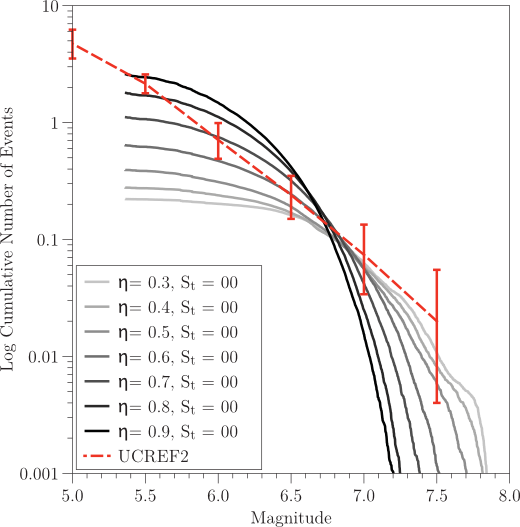
\includegraphics[width=1\textwidth]{graphics/tuning_parameters_1}}
\par\end{center}

\begin{center}
\textbf{(a)}
\par\end{center}%
\end{minipage}\hfill{}%
\begin{minipage}[t]{0.48\columnwidth}%
\begin{center}
\subfloat{\noindent \centering{}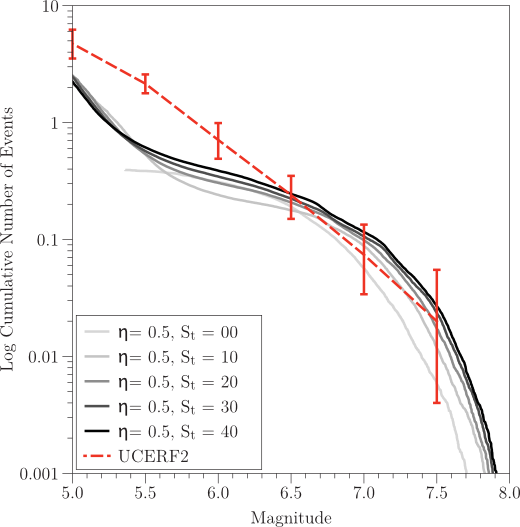
\includegraphics[width=1\textwidth]{graphics/tuning_parameters_2}}
\par\end{center}

\begin{center}
\textbf{(b)}
\par\end{center}%
\end{minipage}\bigskip{}
\begin{minipage}[t]{0.48\columnwidth}%
\begin{center}
\subfloat{\noindent \centering{}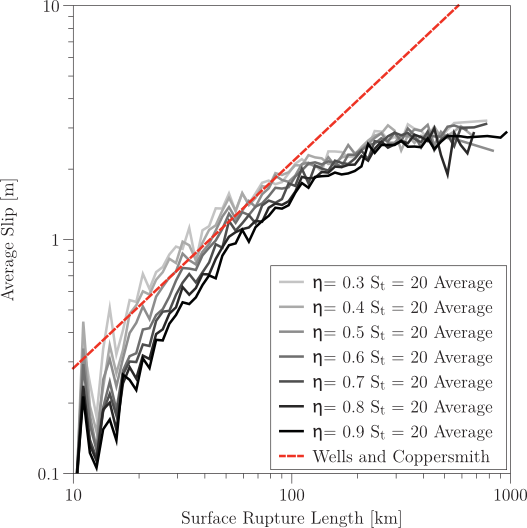
\includegraphics[width=1\textwidth]{graphics/tuning_parameters_3}}
\par\end{center}

\begin{center}
\textbf{(c)}
\par\end{center}%
\end{minipage}\hfill{}%
\begin{minipage}[t]{0.48\columnwidth}%
\begin{center}
\subfloat{\noindent \centering{}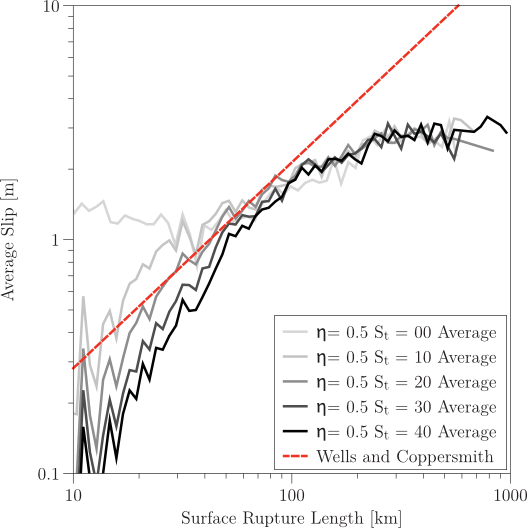
\includegraphics[width=1\textwidth]{graphics/tuning_parameters_4}}
\par\end{center}

\begin{center}
\textbf{(d)}
\par\end{center}%
\end{minipage}

\caption{The output from several VC simulations over a range of dynamic triggering
and slip-scaling threshold parameter values: (a) frequency-magnitude
varying$\eta$; (b) frequency-magnitude varying $S_t$; (c) average
slip-surface rupture length varying $\eta$; and (d) average slip-surface
rupture length varying $S_t$. The dashed red line and error bars
in (a) and (b) are the observed seismicity in California and 95\%
confidence levels as reported by UCERF2 \cite{UCERF2}. The dashed
red lines in (c) and (d) are observed relationships reported by Wells
and Coppersmith \cite{Wells01081994}. \label{fig:tuning_parameters}}
\end{figure}

\par\end{center}


\subsection{Simulation Performance and Scaling\label{sec:element_size_discussion}}

Virtual California is inherently designed to support parallel computing
and this section gives some quantitative results of deploying VC in
multiprocessing environments. It turns out that the key quantities
determining the scope of the output and the simulation performance
are the number and size of the fault elements in the fault model.
The size of the meshed elements will affect both simulation accuracy
and computational resource requirements. The appropriate size of fault
elements for a given simulation depends on the desired minimum earthquake
magnitude and the available computational resources. 


\subsection{Element Size and Minimum Magnitude}

The relationship between element size and minimum magnitude is given
by:

\begin{equation}
M_{min}=\frac{2}{3}log_{10}(1e7\mu sL^{2})-10.7
\end{equation}


where $\mu$ is the Lam� parameter, s is the minimum slip distance,
and $L$ is the element size in meters. The minimum slip distance,
s, will depend on the orientation of the element, the total fault
size, and the interaction with other elements in the system, but will
generally range from approximately 0.1 to 1.0 meters. For example,
for the 12km x 12km fault described in Section \ref{sec:define_mesh_faults}
the minimum slip distance is 0.3 meters. Figure \ref{fig:min_magnitude_elem_size}
shows the relationship in VC between element size and minimum earthquake
magnitude.

\begin{figure}
\subfloat[\label{fig:operations_per_element}Operations required to calculate
a single element-element stress interaction.]{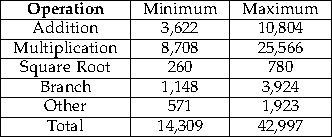
\includegraphics[bb=0bp -22bp 160bp 44bp,width=0.48\textwidth]{graphics/Heien_Sachs_12_number_of_operations}

}\hfill{}\subfloat[\label{fig:min_magnitude_elem_size}Element size versus minimum event
magnitude.]{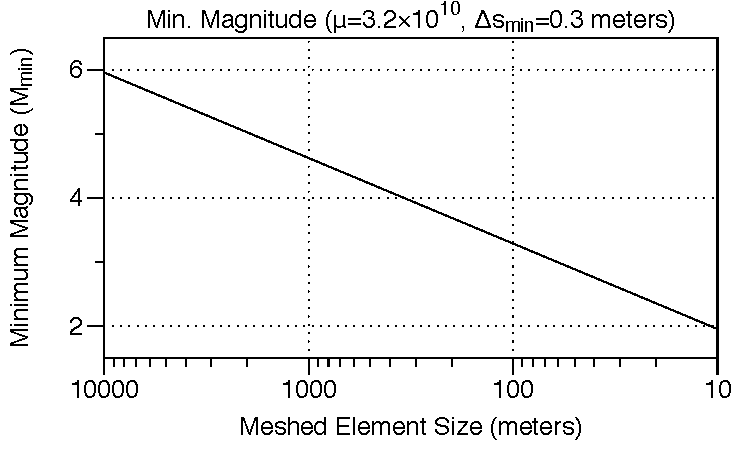
\includegraphics[width=0.48\textwidth]{graphics/min_magnitude}

}

\caption{Number of elements determines computational cost. Element size governs
simulated earthquake magnitude range.}
\end{figure}



\subsection{Element Size and Required Memory}

The number of elements in a model will also affect the required memory.
Since VC uses a Barnes-Hut style approximation algorithm for fault
interaction the actual memory required will depend on the accuracy
of the approximation. For non-approximated fault interaction in a
model with $N$ elements, the memory requirements are:

\begin{equation}
Memory=16N^{2}bytes
\end{equation}


Because the degree of approximation possible with Barnes-Hut will
vary depending on the system geometry it is not possible to give a
function for memory requirements. 

\begin{figure}
\subfloat[\label{fig:memory_vs_element_size_1}Element size determines computational
regime.]{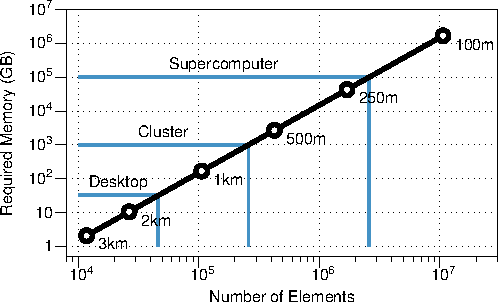
\includegraphics[width=0.48\textwidth]{graphics/Heien_Sachs_12_elements_vs_memory}

}\hfill{}\subfloat[\label{fig:memory_vs_element_size_2}Number of elements vs. memory
requirements with approximations.]{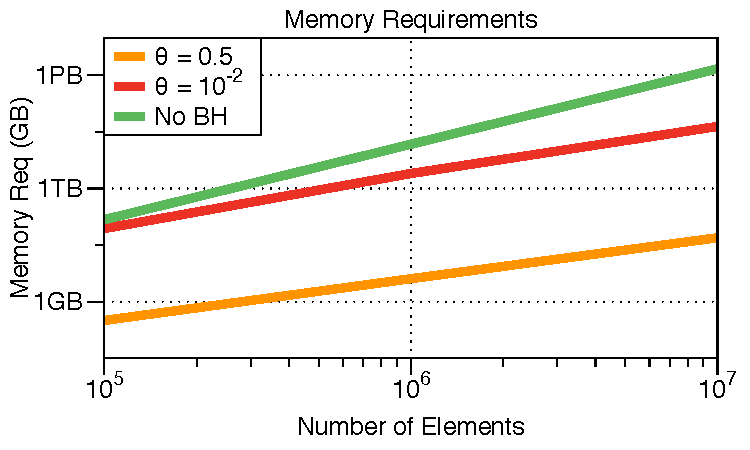
\includegraphics[bb=0bp -12bp 360bp 204bp,width=0.48\textwidth]{graphics/memory_reqs}

}

\caption{Tradeoffs in element size and resource requirements.}
\end{figure}



\subsection{Parallel Performance}

The program flow in Figure \ref{fig:simulation_flow} shows three
main communication points. The global nature of these communications
is a serious bottleneck to simulation performance on a parallel system. 

Figure \ref{fig:sim_breakdown} shows simulation run times for a 13,398
element 100,000 year simulation on a simple cluster system using different
numbers of processors. The cluster has 16 nodes, with two 2.4 GHz
quad-core Xeon processors per node and a Gigabit ethernet network.
For a single processor, most of the time is spent in the long term
stress calculation and the initial Green\textquoteright{}s function
calculations. As the number of processors increases these calculations
scale well but the time spent in communi- cation significantly rises.
By 16 processors the majority of simulation time is spent communicating
and there is very poor strong scalability.

Figure \ref{fig:sim_comm_breakdown} shows the breakdown in time for
different types of communication. For all numbers of processors, the
majority of time is spent distributing stress values over the processors.
This is required because the changes in stress during a rupture potentially
lead to other elements rupturing. However, at a given rupture propagation
step it is highly unlikely the rupture will spread a significant distance
past where it already has traveled.

\begin{figure}
\subfloat[\label{fig:sim_breakdown}Parallel simulation time breakdown.]{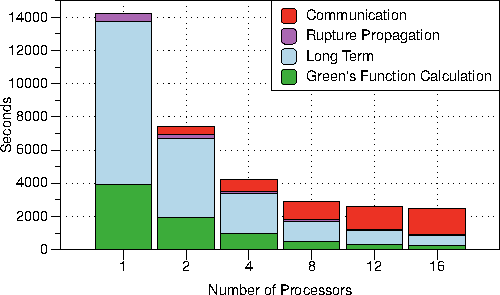
\includegraphics[width=0.48\textwidth]{graphics/Heien_Sachs_12_parallel_sim_time_breakdown}

}\hfill{}\subfloat[\label{fig:sim_comm_breakdown}Parallel communication time breakdown.]{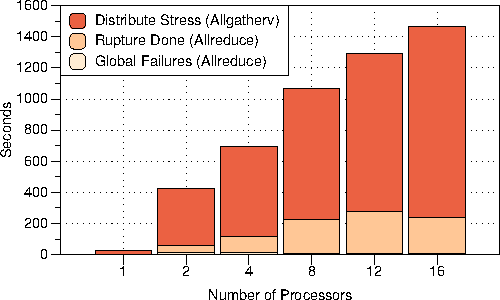
\includegraphics[width=0.48\textwidth]{graphics/Heien_Sachs_12_parallel_comm_time_breakdown}

}

\caption{Breakdown of total simulation time. }
\end{figure}



\chapter{Tutorials \label{cha:Cookbooks}}


\section{Overview}

These tutorials are meant to serve as a guide to some of the types
of problems VC can solve. These cookbook examples are distributed
with the package under the \texttt{examples} directory. However, you
might need to edit these example scripts slightly to launch the job
on your cluster. Each tutorial is a self-contained lesson in how to
use Virtual California. The tutorials increase in degree of complexity
from one to the next.


\subsection{Prerequisites}

Before you begin any of the tutorials, you will need to install Virtual
California following the instructions in Chapter \vref{cha:Installation}.
If you do not wish to create your own mesh at this time, the meshes
are also provided as part of the tutorial. 


\section{Building a Fault Model\label{sec:building_faults}}

Currently, VC uses a simple mesher program for fault model file manipulation.
Mesher imports one or more files (e.g. a trace file), manipulates
them based on user arguments and exports one or more files to be used
as input parameter files for a VC simulation. After following install
instructions in Section \ref{sec:Install}, the mesher program is
compiled to an executable located in VirtualCalifornia/build/src/.
This program is called by the shell scripts in the examples below
to generate a fault model for VC. See section \vref{cha:Appendix-C:Mesher_Parameters}
for more information on the options for the mesher program.

Before using the mesher program, the next sections with give examples
and describe the model files that the mesher creates. For both files,
each commented line describes the parameter in the corresponding column
of the uncommented line immediately following the comments. See section
\vref{cha:Appendix-A:-Input} and section \vref{sec:Trace-File-Format}
for more information on the input fault model files and parameters.


\subsection{Trace File}

The basic outline for creating a fault trace file is given in section
\vref{sec:Fault_model}. The trace file specifies the fault geometry
and physical parameters, and exmple is printed below.
\begin{lyxcode}
\#~Number~of~sections~

\#~Number~of~elements~

\#~Number~of~vertices~

1~1~3~

\#~id:~Unique~ID~of~the~section.~

\#~fault\_id:~ID~of~the~parent~fault.~

\#~name:~Name~of~the~fault.~

\#~id~fault\_id~name~~

0~0~One\_Fault\_Example~

\#~id:~Unique~ID~of~the~element.~

\#~section\_id:~ID~of~the~section~associated~with~the~element.~

\#~vertex\_0:~ID~of~vertex~0.~

\#~vertex\_1:~ID~of~vertex~1.~

\#~vertex\_2:~ID~of~vertex~2.~

\#~is\_quad:~Whether~the~vertices~constitute~3~points~of~a~triangle~(zero)~or~3~points~of~a~parallelogram~(non-zero).~

\#~slip\_rate:~Long~term~slip~rate~of~element~in~meters~per~second.~

\#~aseismic:~Fraction~of~slip~on~element~that~is~aseismic.~

\#~rake:~Rake~angle~of~element~in~radians.~

\#~lame\_mu:~Lame's~parameter~describing~the~shear~modulus~of~the~material~for~this~element~(Pascals).~

\#~lame\_lambda:~Lame's~lambda~parameter~of~the~material~for~this~element,~in~Pascals.~

\#~id~section\_id~vertex\_0~vertex\_1~vertex\_2~is\_quad~slip\_rate~aseismic~rake~lame\_mu~lame\_lambda

0~0~0~1~2~1~3.16881e-10~0~3.14159~3e+10~3.2e+10~

\#~id:~Unique~ID~of~the~vertex.~

\#~latitude:~Latitude~of~the~vertex.~

\#~longitude:~Longitude~of~the~vertex.~

\#~altitude:~Altitude~of~the~vertex~in~meters~(negative~is~below~ground).~

\#~das:~Vertex~distance~along~fault~strike~in~meters.~

\#~id~latitude~longitude~altitude~das~~

0~0~0~0~0

1~6.63961e-18~0~-12000~0~

2~6.6452e-18~0.107798~0~12000
\end{lyxcode}

\subsubsection{Example Traces}

The VirtualCalifornia/examples/fault\_traces/ folder contains the
sample fault traces used in the examples below. In addition, we provide
trace files for all of California's major fault sections in the subfolder
named fault\_traces/ca\_traces/.


\subsection{Friction File\label{sec:Friction_file}}

Virtual California requires one more input file regarding the strengths
of the fault elements. An example friction file is shown below.
\begin{lyxcode}
101~EQSim\_Input\_Friction\_2~1~

111~Fault~friction~from~Ward~All-California~model~

102~End\_Metadata~

120~200~summary~4~~~~Record~200:~Fault~friction~summary,~4~fields

121~1~n\_element~1~~~~Field~1:~Total~number~of~elements~in~the~file~

121~2~elastic\_flag~1~~~~Field~2:~1~if~elastic~parameters~(record~201)~are~included,~0~if~not~

121~3~strength\_flag~1~~~~Field~3:~1~if~fault~strength~(record~202)~is~included,~0~if~not~

121~4~rate\_state\_flag~1~~~~Field~4:~1~if~rate-state~parameters~(record~203)~are~included,~0~if~not~

120~201~elastic\_param~2~~~~Record~201:~Elastic~parameters~

121~1~lame\_lambda~2~~~~Field~1:~Lame~modulus~lambda~(Pascal)~

121~2~lame\_mu~2~~~~Field~2:~Lame~modulus~mu,~also~known~as~the~shear~modulus~(Pascal)~

120~202~fault\_strength~3~~~~Record~202:~Fault~strength~

121~1~index~1~~~~Field~1:~Element~index~number~(consecutive~integers,~starting~with~1)~

121~2~static\_strength~2~~~~Field~2:~Element~static~yield~strength~(Pascal)~

121~3~dynamic\_strength~2~~~~Field~3:~Element~dynamic~sliding~strength~(Pascal)~

120~203~rate\_state~6~~~~Record~203:~Rate-state~parameters~

121~1~index~1~~~~Field~1:~Element~index~number~(consecutive~integers,~starting~with~1)~

121~2~A~2~~~~Field~2:~Element~rate-state~parameter~A~

121~3~B~2~~~~Field~3:~Element~rate-state~parameter~B~

121~4~L~2~~~~Field~4:~Element~rate-state~characteristic~distance~L~(meters)~

121~5~f0~2~~~~Field~5:~Element~rate-state~friction~coefficient~f0~

121~6~V0~2~~~~Field~6:~Element~rate-state~reference~velocity~V0~(meters/second)~

103~End\_Descriptor~

200~1~1~1~0~

201~~3.200000e+010~~3.000000e+010~

202~1~~2.008100e+007~~0.000000e+000~

999~End
\end{lyxcode}
The static strength for the fault sections in California are given
by Ward's All-California model \cite{Ward01112012}. 


\subsection{Simulation Parameter File}

The main simulation input file is the parameter file. This file tells
the simulator where the fault model files are located, sets various
simulation variables, and specifies the output of the simulation.
The parameter file is generated by the ``setup\_params.sh'' script,
this script is included in VirtualCalifornia/examples/single\_fault/
and VirtualCalifornia/examples/two\_fault/. An example parameter file
is shown below, and the usage of the ``setup\_params.sh'' script is
documented in the following section.
\begin{lyxcode}
sim.version~~~~~~~~~~~~~~~~~=~2.0~

sim.time.end\_year~~~~~~~~~~~=~10000~

sim.greens.method~~~~~~~~~~~=~standard~

sim.greens.use\_normal~~~~~~~=~false~

sim.friction.dynamic~~~~~~~~=~0.5~

sim.file.input~~~~~~~~~~~~~~=~single\_fault\_1000.txt~

sim.file.input\_type~~~~~~~~~=~text~

sim.eqsim.file.friction~~~~~=~single\_friction.dat~

sim.file.output\_event~~~~~~~=~events\_1000.txt~

sim.file.output\_sweep~~~~~~~=~sweeps\_1000.txt~

sim.file.output\_event\_type~~=~text
\end{lyxcode}

\subsection{Producing a Fault Model\label{sec:Using-Mesher}}

There are two final steps to produce a fault model. The first step
uses ``setup\_mesh.sh'' to generate the fault trace file, and the
second step is to edit the simulation parameter file ``params.d''.
This method is illustrated in the tutorials in the following sections.


\subsubsection{Using the Mesher}

The sample Bash shell script that uses the mesher program to generate
the mesh from the fault traces will be located in VirtualCalifornia/examples/single\_fault/
(or two\_fault/) and is named ``setup\_mesh.sh''. The syntax for using
this is:
\begin{lyxcode}
\$~bash~setup\_mesh.sh~ELEM\_SIZE~TAPER\_METHOD
\end{lyxcode}
The required (bold) arguments are described below.
\begin{lyxcode}
ELEM\_SIZE~~~~~~=~the~size~of~the~square~fault~elements~in~meters

TAPER\_METHOD~~~=~none,~taper,~or~taper\_norm~(see~section~\ref{sec:Trace-File-Format})~
\end{lyxcode}
This script takes the trace file from the previous section, as well
as other keyword arguments described in section \ref{cha:Appendix-C:Mesher_Parameters},
and creates several simulation files in a subfolder named by the TAPER\_METHOD.
Below is an example script that calls the mesher, gives it a previously
created trace file, instructs the mesher to return several files,
and tells the mesher to merge doubly named vertices in the trace file.


\subsubsection{Parameter File}

Simply copy the ``params.d'' file into the subfolder generated by
the mesher. Edit the file so the simulation parameters are set correctly
for the current run. 


\section{Single Element Tutorial\label{sec:Tutorial_single}}


\subsection{Overview}

This tutorial is the simplest possible implementation of Virtual California.
In this tutorial we will build the trace file for a single vertical
strike-slip fault element, then use this to build a fault model with
the mesher program. We will run this simulation for 10,000 years and
then test and explore the output. 


\subsection{Creating Input Files}

We are going to create a new fault trace file for this single element.
The only data we need for this are the latitude and longitude of the
endpoints of our element. For this example let's use the following
coordinates (37.83,-122.4797) and (37.803,-122.4765). These endpoints
give a 3km fault element than runs parallel and directly under the
Golden Gate Bridge in San Francisco. The trace file is printed below
and the fault element is shown above ground in figure \ref{fig:Golden_Gate_single}.
\begin{lyxcode}
\#~fault\_id:~ID~number~of~the~parent~fault~of~this~section~

\#~num\_points:~Number~of~trace~points~comprising~this~section~

\#~section\_name:~Name~of~the~section~

0~2~One\_Fault\_GG\_Example~

\#~latitude:~Latitude~of~trace~point~

\#~longitude:~Longitude~of~trace~point~

\#~altitude:~Altitude~of~trace~point~(meters)~

\#~depth\_along\_dip:~Depth~along~dip~(meters)~

\#~slip\_rate:~Slip~rate~at~trace~point~(centimeters/year)~

\#~aseismic:~Fraction~of~slip~that~is~aseismic~at~point~

\#~rake:~Fault~rake~at~trace~point~(degrees)~

\#~dip:~Fault~dip~at~trace~point~(degrees)~

\#~lame\_mu:~Lame's~mu~parameter~at~trace~point~(Pascals)~

\#~lame\_lambda:~Lame's~lambda~parameter~at~trace~point~(Pascals)~

37.85~~~-122.482~0~3000~1~0~180~90~3e+10~3.2e+10~

37.7425~-122.47~~0~3000~1~0~180~90~3e+10~3.2e+10
\end{lyxcode}
To create the input files, we use the mesher program as follows (arguments
explained in section \ref{sec:building_faults}).
\begin{lyxcode}
\$~cd~examples/single\_fault/

\$~bash~setup\_mesh.sh~3000~none
\end{lyxcode}
Which generates several output files as listed by the command line
output shown below.
\begin{lyxcode}
{*}{*}{*}~Summary~of~edits~{*}{*}{*}~

File~import~../../fault\_traces/single\_fault\_trace.txt~with~type~trace...~done.~

File~export~single\_fault\_3000.txt~with~type~text...~done.~

File~export~single\_fault\_3000.kml~with~type~kml...~done.~

Print~statistics~to~statistics\_3000.txt
\end{lyxcode}
\begin{figure}
\centering{}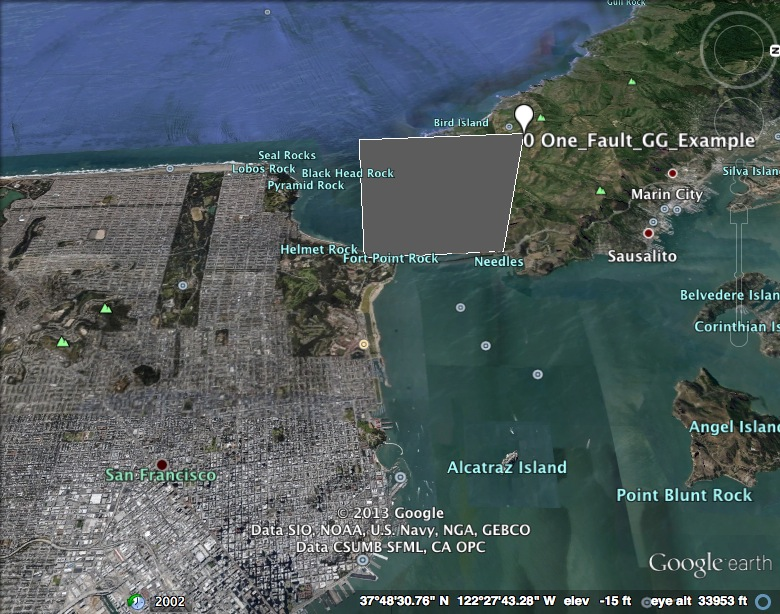
\includegraphics[bb=0bp 0bp 780bp 614bp,width=0.72\textwidth]{graphics/One_Fault_Golden_Gate}\caption{\label{fig:Golden_Gate_single}Single 3km x 3km fault element running
under the Golden Gate Bridge in San Francisco, shown above ground.
This plot was generated by Google Earth from the KML file that the
mesher program created from the trace file.}
\end{figure}


We will also need a friction file that specifies the failing stress
for each fault element. For this example we will use the file printed
in section \ref{sec:Friction_file}. 

Values for the faults in California are taken from Ward's ALLCAL2
model \cite{Ward01112012}, more information at \href{http://scec.usc.edu/research/eqsims/documentation.html}{http://scec.usc.edu/research/eqsims/documentation.html}. 


\subsection{Assimilating Input Files}

Now, from the same directory (examples/single\_fault/) we need to
edit the parameter file, and place the VC executable and input files
into the same directory.
\begin{lyxcode}
\$~bash~setup\_params.sh~3000~none~0.5



dynamic~triggering~factor:~~~0.5~

taper~method:~~~~~~~~~~~~~~~~none~

element~size~{[}m{]}:~~~~~~~~~~~~3000~

{*}{*}{*}{*}parameter~file~written:~~none/params\_3000.d
\end{lyxcode}
The next thing is to copy the compiled VC executable into the same
directory as our parameter files.
\begin{lyxcode}
\$~cp~../../build/src/vc~./none/
\end{lyxcode}
The simulation parameter file was created in the /single\_fault/none/
directory and should match what is printed below. 
\begin{lyxcode}
sim.version~~~~~~~~~~~~~~~~~~~~~=~2.0~

sim.time.end\_year~~~~~~~~~~~~~~~=~10000~

sim.greens.method~~~~~~~~~~~~~~~=~standard~

sim.greens.use\_normal~~~~~~~~~~~=~false~

sim.friction.dynamic~~~~~~~~~~~~=~0.5~

sim.file.input~~~~~~~~~~~~~~~~~~=~single\_fault\_3000.txt~

sim.file.input\_type~~~~~~~~~~~~~=~text~

sim.eqsim.file.friction~~~~~~~~~=~../single\_friction.dat~

sim.file.output\_event~~~~~~~~~~~=~events\_3000.txt~

sim.file.output\_sweep~~~~~~~~~~~=~sweeps\_3000.txt~

sim.file.output\_event\_type~~~~~~=~text
\end{lyxcode}

\subsection{Running VC}

Now that we have generated the fault mesh and put all the simulation
files in one place, we are now ready to run the simulation. Run this
simulation by simply executing the vc executable and passing the parameter
file as a command line argument:
\begin{lyxcode}
\$~cd~./none/
\end{lyxcode}
\$ ./vc ./params\_3000.d


\section{Tutorial Using Multiple Elements\label{sec:Tutorial_multiple}}


\subsection{Overview }

Now we are going to repeat the single vertical strike-slip fault tutorial
from the previous section, but we will break up the fault into multiple
elements. 


\subsection{Creating Input Files}

We simply need to change the element size when we call the mesher
program. To protect the previous example, first we need to edit the
``setup\_mesh.sh'' file so that we write the files to a new directory.
In the script, just make this change: DIR\_NAME=Golden\_Gate\_Example\_Multiple.
Then we generate the mesh with the following commands.
\begin{lyxcode}
\$~cd~examples/single\_fault/

\$~bash~setup\_mesh.sh~1000~none~
\end{lyxcode}
Which should output the following.
\begin{lyxcode}
{*}{*}{*}~Summary~of~edits~{*}{*}{*}~

File~import~../../fault\_traces/single\_fault\_trace.txt~with~type~trace...~done.~

File~export~single\_fault\_1000.txt~with~type~text...~done.~

File~export~single\_fault\_1000.kml~with~type~kml...~done.~

Print~statistics~to~statistics\_1000.txt
\end{lyxcode}
However, we cannot use the same friction file. We have more fault
elements this time and the friction parameters must be specified for
each element. For this simple example we will have the same failing
stress for all the elements since they are part of the same local
fault section and thus are likely to have the same physical properties.
\begin{lyxcode}
\$~bash~setup\_params.sh~1000~none~0.5~



dynamic~triggering~factor:~~~0.5~

taper~method:~~~~~~~~~~~~~~~~none~

element~size~{[}m{]}:~~~~~~~~~~~~1000~

{*}{*}{*}{*}parameter~file~written:~~none/params\_1000.d~
\end{lyxcode}
After executing this, we still need to make one more change to the
parameter file. We need to use new friction file, named ``multiple\_friction\_uniform.dat''.
So we need to edit the ``single\_fault/none/params\_1000.d'' so the
simulation will know to use the multiple element friction file. After
the edits the parameter file should match what is printed below.
\begin{lyxcode}
sim.version~~~~~~~~~~~~~~~~~~~~~~~=~2.0~

sim.time.end\_year~~~~~~~~~~~~~~~~~=~10000~

sim.greens.method~~~~~~~~~~~~~~~~~=~standard~

sim.greens.use\_normal~~~~~~~~~~~~~=~false~

sim.friction.dynamic~~~~~~~~~~~~~~=~0.5~

sim.file.input~~~~~~~~~~~~~~~~~~~~=~single\_fault\_1000.txt~

sim.file.input\_type~~~~~~~~~~~~~~~=~text~

sim.eqsim.file.friction~~~~~~~~~~~=~../multiple\_friction\_uniform.dat

sim.file.output\_event~~~~~~~~~~~~~=~events\_1000.txt~

sim.file.output\_sweep~~~~~~~~~~~~~=~sweeps\_1000.txt~

sim.file.output\_event\_type~~~~~~~~=~text
\end{lyxcode}
\begin{figure}
\centering{}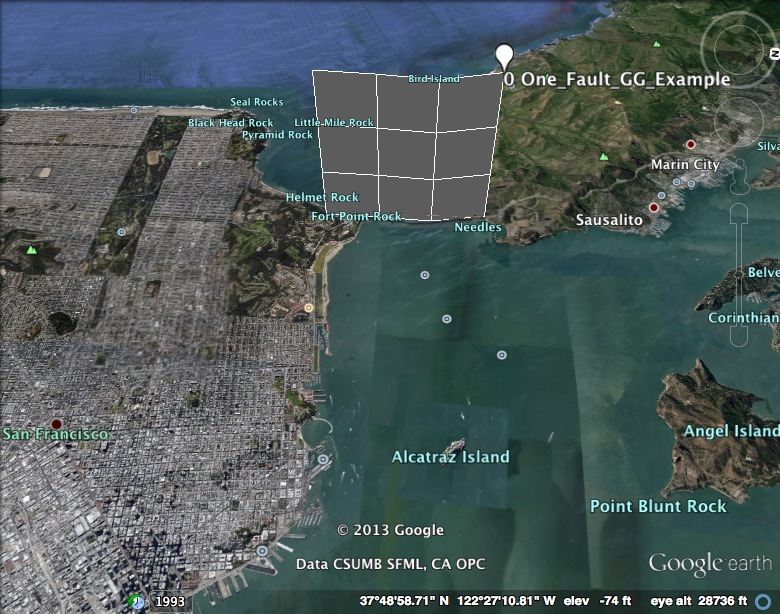
\includegraphics[width=0.72\textwidth]{graphics/Golden_Gate_Multi_Element}\caption{\label{fig:Golden_Gate_multiple}The same 3km x 3km fault section
from figure \ref{fig:Golden_Gate_single} but meshed into 1km x 1km
elements. This plot was generated by Google Earth from the KML file
that the mesher program created using the trace file.}
\end{figure}



\subsection{Assimilating Input Files}

Now lets navigate to the newly created directory and assimilate our
simulation files. The only difference is that since the VC executable
is a large file, we will just move it over from the previous example's
directory.
\begin{lyxcode}
\$~cd~./none/

\$~mv~../single\_fault/none/vc~./
\end{lyxcode}

\subsection{Running VC}

Again we run the simulation by simply executing the vc executable:
\begin{lyxcode}
\$~./vc~./params\_1000.d
\end{lyxcode}

\section{Multiple Fault Sections}


\subsection{Overview}

This tutorial will explore a Virtual California simulation involved
two neighboring fault sections --- each 15km long and 12km deep meshed
into 3km by 3km elements. We will also use larger fault elements than
the previous example, which raises the lower bound for magnitudes
in the output data set. Furthermore, we now will be simulating the
interaction between 40 elements so the computational resource requirements
grow as well (see section \ref{sec:element_size_discussion} for a
detailed discussion).


\subsection{Input Files}

We will use another trace file that is provided with a VC install.
This trace file specifies two neighboring vertical strike slip fault
sections that intersect at the Earth and Physical Sciences building
on campus at the University of California, Davis, shown in figure
\ref{fig:Davis_2_fault}. We generate the mesh with the following
commands.
\begin{lyxcode}
\$~cd~examples/two\_fault/

\$~bash~setup\_mesh.sh~3000~none~
\end{lyxcode}
Which should output the following.
\begin{lyxcode}
{*}{*}{*}~Summary~of~edits~{*}{*}{*}

File~import~../../fault\_traces/multiple\_fault\_trace.txt~with~type~trace...~done.~

File~export~Davis\_multiple\_3000.txt~with~type~text...~done.~

File~export~Davis\_multiple\_3000.kml~with~type~kml...~done.~

Print~statistics~to~statistics\_3000.txt
\end{lyxcode}
Next we will generate the parameter file.
\begin{lyxcode}
\$bash~setup\_params.sh~3000~none~0.5



dynamic~triggering~factor:~~0.5~

taper~method:~~~~~~~~~~~~~~~none~

element~size~{[}m{]}:~~~~~~~~~~~3000~

{*}{*}{*}{*}parameter~file~written:~none/params\_3000.d~
\end{lyxcode}
We will be using a supplied friction file for this example. This friction
file gives each element a slightly different failure stress, to ensure
that the faults do not simply act like one large fault element.

\begin{figure}
\centering{}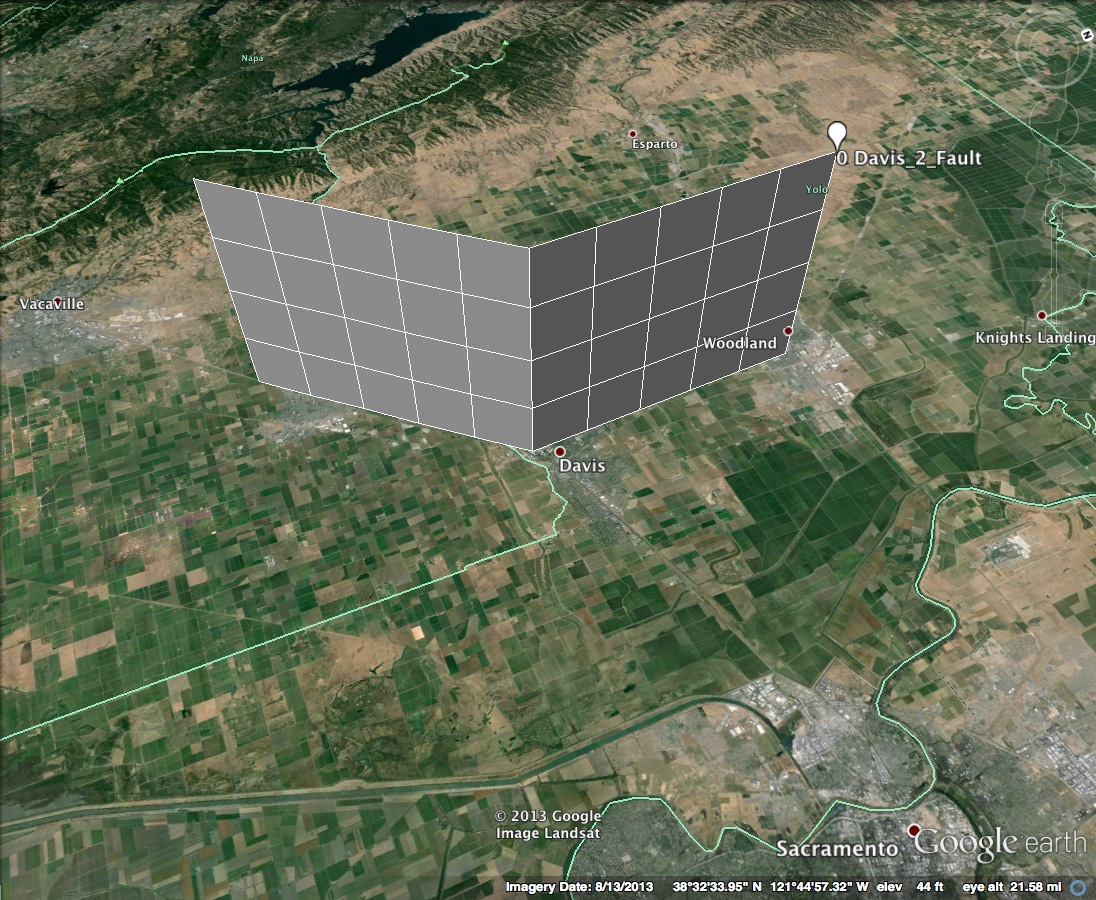
\includegraphics[bb=0bp 0bp 1096bp 900bp,width=0.72\textwidth]{graphics/Davis_2_Fault}\caption{\label{fig:Davis_2_fault}Two fault sections that meet at the UC Davis
campus. The fault sections are 15km x 12km and meshed into 3km x 3km
elements. This plot was generated by Google Earth from the KML file
that the mesher program created using the trace file.}
\end{figure}



\subsection{Assimilating Input Files}

Now lets navigate to the newly created directory and assimilate our
simulation files. The caveat is that since the VC executable is a
large file, we will just move it over from the previous example's
directory instead of making multiple copies from VirtualCalifornia/build/src/vc.
\begin{lyxcode}
\$~cd~./none/

\$~mv~../single\_fault/none/vc~./
\end{lyxcode}

\subsection{Running VC}

Again we run the simulation by simply executing the vc executable:
\begin{lyxcode}
\$~./vc~./params\_3000.d
\end{lyxcode}

\part{Appendices}

\appendix

\chapter{\label{cha:Appendix-A:-Input}Input Parameters for Virtual California}


\section{Input Parameters Grouped by Functionality}

This section explains the meaning of the input parameters for Virtual
California. These parameters are grouped by their functionality. Parameters
are given with their default values.


\subsection{Simulation time parameters}

\noindent %
\begin{tabular}{|>{\raggedright}p{2.3in}|>{\raggedright}p{3.8in}|}
\hline 
\texttt{\small{sim.time.start\_year = 0}} & The starting year of the simulation\tabularnewline
\hline 
\texttt{\small{sim.time.end\_year = 1000}} & The ending year of the simulation.\tabularnewline
\hline 
\end{tabular}


\subsection{\noindent System Parameters}

\noindent %
\begin{tabular}{|>{\raggedright}p{2.3in}|>{\raggedright}p{3.8in}|}
\hline 
\texttt{\small{sim.system.rawfile.lat0 = 31.5}}{\small \par}

\texttt{\small{sim.system.rawfile.lon0 = -126}} & Base latitude and longitude for coordinates of meshed model. These
values are used in the conversion from This should be roughly within
the bounds of your fault model to avoid warping from conversion to
a Cartesian coordinate system. If undefined, defaults to (-126.0,
31.5) (about 500 miles W-SW from Los Angeles).\tabularnewline
\hline 
\texttt{\small{sim.system.kill\_cff}} & Below what CFF a fault will be deactivated. Certain fault configurations
can have stress sinks, and this parameter will effectively remove
them. If undefined, defaults to being turned off (negative infinity).\tabularnewline
\hline 
\texttt{\small{sim.system.sanity\_check = false}} & Whether to perform sanity checks on simulation values and abort if
any values are outside acceptable ranges.\tabularnewline
\hline 
\texttt{\small{sim.system.transpose\_matrix = true}} & Whether to store the Green's matrix in a transposed form to significantly
improve performance. This should only be set to false for performance
profiling.\tabularnewline
\hline 
\texttt{\small{sim.system.progress\_period = 0}} & How frequently (in real seconds) to display simulation progress. If
undefined or \textless{}= 0, simulation progress will not be displayed.\tabularnewline
\hline 
\texttt{\small{sim.system.depth\_dependent\_slip = false}} & Whether the fault velocity (slip rate) should be altered by depth.
This is based on the equation $v=v_{s}(1-(\frac{z}{d})^{2})$ where
$v_{s}$ is the original long term slip velocity, $d$ is the total
fault depth, and $z$ is the depth of the block center.\tabularnewline
\hline 
\texttt{\small{sim.system.checkpoint\_period}} & How frequently (in simulation events) a checkpoint is saved. If undefined
or \textless{}= 0, checkpoints will not be saved.\tabularnewline
\hline 
\texttt{\small{sim.system.checkpoint\_prefix = sim\_state\_}} & The prefix of the state save files, which will also include the event
count.\tabularnewline
\hline 
\end{tabular}


\subsection{Friction parameters}

\begin{tabular}{|>{\raggedright}p{2.3in}|>{\raggedright}p{3.8in}|}
\hline 
\texttt{\small{sim.friction.dynamic}} & The dynamic rupture value to use in the simulation from 0 to 1. Higher
values indicate ruptures are more likely to propagate along a fault
and result in larger earthquakes, while lower values indicate ruptures
are less likely to propagate and result in smaller earthquakes. If
undefined or outside the allowed range, use the dynamic values specified
for each fault element.\tabularnewline
\hline 
\texttt{\small{sim.friction.law = original}} & Either use the \texttt{\small{original}} or \texttt{\small{stepped}}
friction law.\tabularnewline
\hline 
\texttt{\small{sim.friction.slip\_scaling\_threshold = 10}} & The slip scaling threshold parameter used to scale slip with rupture
size as per Equation \ref{eq:sst_one}.\tabularnewline
\hline 
\end{tabular}


\subsection{Green's function parameters}

\begin{tabular}{|>{\raggedright}p{2.3in}|>{\raggedright}p{3.8in}|}
\hline 
\texttt{\small{sim.greens.method = standard}} & The method to calculate the Green's functions for fault element stress
interactions. There are three possible choices for this parameter
- \texttt{\small{standard}}, \texttt{\small{bh}} and \texttt{\small{file}}.
The \texttt{\small{standard}} option will calculate the Green's functions
using the normal Okada equations with all element-element interactions.
The \texttt{\small{bh}} option will use a Barnes Hut style approximation.
The \texttt{\small{file}} option will read precalculated values from
an input file (specified using \texttt{\small{sim.greens.input}}).\tabularnewline
\hline 
\texttt{\small{sim.greens.bh\_theta = 0.0}} & Parameter for Barnes Hut calculation of Green's function (between
0 and 1). Lower values mean less of an approximation. If undefined,
defaults to 0 (meaning it effectively doesn't use Barnes Hut approximation).\tabularnewline
\hline 
\texttt{\small{sim.greens.input}} & If \texttt{\small{sim.greens.method}} is defined as \texttt{\small{file}},
this is the name of the HDF5 file to read the Green's function values
from.\tabularnewline
\hline 
\texttt{\small{sim.greens.output}} & The name of the HDF5 file to write the Green's function values to.\tabularnewline
\hline 
\texttt{\small{sim.greens.use\_normal = true}} & Whether to use the Green's normal stress function in calculations
or just the Green's shear function.\tabularnewline
\hline 
\texttt{\small{sim.greens.kill\_distance = 0.0}} & Kills interaction between any two blocks greater than this distance
(in km) apart. If undefined or \textless{}= 0, all interactions will
remain the same.\tabularnewline
\hline 
\end{tabular}


\subsection{File name parameters}

\begin{tabular}{|>{\raggedright}p{2.3in}|>{\raggedright}p{3.8in}|}
\hline 
\texttt{\small{sim.file.system\_output}} & The system file of the simulation. If undefined, no system information
file will be written.\tabularnewline
\hline 
\texttt{\small{sim.file.events}} & The file which events will be written to. If undefined, events will
not be recorded in an ASCII format.\tabularnewline
\hline 
\texttt{\small{sim.file.hdf5\_output}} & The file to write HDF5 formatted simulation and event data into. If
undefined, HDF5 data will not be recorded.\tabularnewline
\hline 
\end{tabular}


\subsection{EqSim File Parameters}

\begin{tabular}{|>{\raggedright}p{2.3in}|>{\raggedright}p{3.8in}|}
\hline 
\texttt{\small{sim.eqsim.file.output}} & The file which EqSim style event logging will be written to. If undefined,
the EqSim events file will not be created.\tabularnewline
\hline 
\texttt{\small{sim.eqsim.file.condition}} & The file to read EqSim style initial condition information from. If
undefined, initial shear and normal stresses will be 0 and rhogd will
be 1.557e8.\tabularnewline
\hline 
\texttt{\small{sim.eqsim.file.friction}} & The file to read EqSim style friction information from. If undefined,
EqSim input files will not be used.\tabularnewline
\hline 
\texttt{\small{sim.eqsim.file.geometry}} & The file to read EqSim style geometry information from. If undefined,
EqSim input files will not be used.\tabularnewline
\hline 
\texttt{\small{sim.eqsim.file.slipmap\_mag = 7.5}} & The magnitude cutoff to print slip maps in the EqSim event file.\tabularnewline
\hline 
\end{tabular}


\subsection{\noindent Noise parameters}

\noindent %
\begin{tabular}{|>{\raggedright}p{2.3in}|>{\raggedright}p{3.8in}|}
\hline 
\texttt{\small{sim.noise.event = 0.0}} & Noise in single stress drop events.\tabularnewline
\hline 
\texttt{\small{sim.noise.slip\_deficit = 0.0}} & Noise in initial slip\_deficit.\tabularnewline
\hline 
\texttt{\small{sim.noise.stress.stress = 0.0}} & Noise applied to stress drop at start of simulation (affects all of
simulation).\tabularnewline
\hline 
\texttt{sim.noise.}\texttt{\small{resolution}}\texttt{ = 10.0} & Stress noise resolution in km (over what range to apply a single noise
value)\tabularnewline
\hline 
\end{tabular}


\subsection{BASS (Branching Aftershock Sequence) model parameters}

\begin{tabular}{|>{\raggedright}p{2.3in}|>{\raggedright}p{3.8in}|}
\hline 
\texttt{\small{sim.bass.max\_generations = 0}} & Maximum number of aftershock generations to generate in BASS model.
If this is 0 then the BASS aftershock model will not be used.\tabularnewline
\hline 


\texttt{\small{sim.bass.mm = 4.0}}{\small \par}

\texttt{\small{sim.bass.dm = 1.25}}{\small \par}

\texttt{\small{sim.bass.b = 1.0}}{\small \par}

\texttt{\small{sim.bass.c = 0.1}}{\small \par}

\texttt{\small{sim.bass.p = 1.25}}{\small \par}

\texttt{\small{sim.bass.d = 300}}{\small \par}

\texttt{\small{sim.bass.q = 1.35}} & Different parameters for BASS model. See paper \cite{Turcotte:2007up}
for details.

Mm: minimum magnitude

dM: strength of aftershock sequence (intensity of aftershocks)

b: scaling of frequency magnitude

c: start of aftershocks in days

p: time decay rate of aftershocks

d: distance parameter for aftershocks in meters

q: distance decay rate\tabularnewline
\hline 
\end{tabular}


\subsection{Parallel simulation parameters}

\noindent %
\begin{tabular}{|>{\raggedright}p{2.3in}|>{\raggedright}p{3.8in}|}
\hline 
\texttt{\small{sim.parallel.spec\_exec = none}} & Choose the type of speculative execution to be used to improve simulation
speed. Currently experimental. Can be either \texttt{\small{none}},
\texttt{\small{fixed}}, or \texttt{\small{adaptive}}. If \texttt{none}
is chosen, speculative execution will not be used. If \texttt{\small{fixed}}
or \texttt{\small{adaptive}} are chosen, the speculative execution
scheme is used with either a fixed boundary distance or adaptive distance.\tabularnewline
\hline 
\texttt{sim.parallel.spec\_exec\_distance = 0} & The boundary distance to use in the \texttt{\small{fixed}} speculative
execution scheme. This affects how frequently the simulation goes
into speculative mode.\tabularnewline
\hline 
\end{tabular}


\chapter{Virtual California Input File Format}


\section{Introduction}

There are several input files used in VC. 


\section{\label{sec:Trace-File-Format}Trace File Format}

The initial fault geometry for VC runs is defined by the trace file.
Each trace file describes a single fault by the location of points
along the fault trace and associated fault characteristics at each
of the points. A single VC model for a simulation can be generated
by combining multiple fault traces using the mesher program (see section
\ref{sec:Tutorial_multiple} for an example).

The trace files are ASCII format with comments indicated by a \# (hash)
mark. Lines that begin with a \# will be ignored and any values after
a \# in a line will be ignored. The initial line in the trace file
outlines the fault described in the file using the following attributes:\vspace*{\bigskipamount}


\noindent %
\begin{tabular}{|>{\raggedright}p{1.85in}|>{\raggedright}p{4.25in}|}
\hline 
\texttt{\small{fault\_id}} & ID number of the parent fault of this section. Used to unify multi-segment
faults defined in separate files.\tabularnewline
\hline 
\texttt{num\_points} & The number of trace points comprising this section.\tabularnewline
\hline 
\texttt{section\_name} & Name of the section, may not contain whitespace.\tabularnewline
\hline 
\end{tabular}

\vspace*{\bigskipamount}
The remainder of the file defines each of the trace points for the
fault. Each trace point is described using the following attributes.
The units of the attributes in the file were chosen to be easily human
understandable, however in the simulation they are converted to SI
units.\vspace*{\bigskipamount}


\noindent %
\begin{tabular}{|>{\raggedright}p{1.85in}|>{\raggedright}p{4.25in}|}
\hline 
\texttt{\small{latitude}} & Latitude of trace point (must be in {[}-90, 90{]}).\tabularnewline
\hline 
\texttt{longitude} & Longitude of trace point (must be in {[}-180, 180{]}).\tabularnewline
\hline 
\texttt{altitude} & Altitude of trace point in meters above ground. All faults should
be underground (negative altitude). Faults defined above ground will
have undefined results.\tabularnewline
\hline 
\texttt{depth\_along\_dip} & The depth of the fault along the dip in meters (must be greater than
0). For a dip angle of $\delta$ the actual depth of the fault will
be depth\_along\_dip{*}$\sin \delta$.\tabularnewline
\hline 
\texttt{slip\_rate} & The long term slip rate of the fault in centimeters per year.\tabularnewline
\hline 
\texttt{aseismic} & The fraction of slip that is aseismic (must be in {[}0,1{]}).\tabularnewline
\hline 
\texttt{rake} & The fault rake angle in degrees (must be in {[}-180, 180{]}).\tabularnewline
\hline 
\texttt{dip} & The fault dip angle in degrees (must be in {[}0,90{]}).\tabularnewline
\hline 
\texttt{lame\_mu} & Lame's mu parameter describing material properties in Pascals (must
be greater than 0).\tabularnewline
\hline 
\texttt{lame\_lambda} & Lame's lambda parameter describing material properties in Pascals.\tabularnewline
\hline 
\end{tabular}


\chapter{\label{cha:Appendix-C:Mesher_Parameters}Mesher Program Options}


\section{Mesher Options Grouped by Functionality}

This section explains the meaning of the options used by the mesher
program for Virtual California model file manipulation. These options
are grouped by their functionality. 


\subsection{General Options}

\noindent %
\begin{tabular}{|>{\raggedright}p{3.05in}|>{\raggedright}p{3.05in}|}
\hline 
-s FILE, -\/-print\_statistics=FILE & Print statistics regarding final model to the specified file.\tabularnewline
\hline 
-m, -\/-merge\_duplicate\_verts & Merge duplicate vertices after importing files.\tabularnewline
\hline 
-d, -\/-delete\_unused & Delete unused vertices after importing files.\tabularnewline
\hline 
\end{tabular}


\subsection{\noindent File Import Options}

\noindent %
\begin{tabular}{|>{\raggedright}p{3.05in}|>{\raggedright}p{3.05in}|}
\hline 
-i FILE, -\/-import\_file=FILE & Specify a model file to import and merge. Must have a paired import\_file\_type.\tabularnewline
\hline 
-j TYPE, -\/-import\_file\_type=TYPE & Specify a model file type for importing. Must have a paired import\_file.\tabularnewline
\hline 
-l FILE, -\/-import\_trace\_element\_size=FILE & Specify the element size to use for trace file meshing. Must have
a paired trace type file import.\tabularnewline
\hline 
-t METHOD, -\/-taper\_fault\_method=METHOD & Specify the how to taper the imported trace when meshing. Must have
a paired trace type file import. Choices for taper method are: none,
taper, taper\_renorm. Taper follows the convention of \ref{sec:tapering}.
Taper\_norm adds a constant offset velocity everywhere so element
behavior will more closely resemble observation.\tabularnewline
\hline 
-C FILE, -\/-import\_eqsim\_condition=FILE & Specify an EQSim condition file to import for the model.\tabularnewline
\hline 
-F FILE, -\/-import\_eqsim\_friction=FILE & Specify an EQSim friction file to import for the model.\tabularnewline
\hline 
-G FILE, -\/-import\_eqsim\_geometry=FILE & Specify an EQSim geometry file to import for the model.\tabularnewline
\hline 
\end{tabular}


\subsection{\noindent File Export Options}

\noindent %
\begin{tabular}{|>{\raggedright}p{3.05in}|>{\raggedright}p{3.05in}|}
\hline 
-e FILE, -\/-export\_file=FILE & Specify a file to export the completed model to. Must have a paired
export\_file\_type.\tabularnewline
\hline 
-f TYPE, -\/-export\_file\_type=TYPE & Specify a file type to export the completed model. Must have a paired
export\_file.\tabularnewline
\hline 
-D FILE, -\/-export\_eqsim\_condition=FILE & Specify an EQSim condition file to export for the model.\tabularnewline
\hline 
-R FILE, -\/-export\_eqsim\_friction=FILE & Specify an EQSim friction file to export for the model.\tabularnewline
\hline 
-M FILE, -\/-export\_eqsim\_geometry=FILE & Specify an EQSim geometry file to export for the model.\tabularnewline
\hline 
\end{tabular}


\chapter{\label{chap:Virtual-California-Output}Virtual California Output
File Format}


\section{Introduction}

The format of the output files of Virtual California is described
here. All outputs are in non-dimensional units unless specified.


\section{HDF5 Output}

If Virtual California is compiled with the HDF5 library it is possible
to output simulation results in this format. This format aims to be
a full description of the simulation and results, containing both
a description of the fault system and events that occurred on the
system. In this way the user can write scripts that can read all information
from a single source. The output file is composed of several tables
and datasets describing the input and output to a simulation. Depending
on user options some of these tables may be empty but they will always
exist in the file.


\subsection{About HDF5}

The Hierarchical Data Format (HDF) is a portable file format developed
at the National Center for Supercomputing Applications (NCSA) \url{hdf.ncsa.uiuc.edu/HDF5}.
It is designed for storing, retrieving, analyzing, visualizing, and
converting scientific data. The current and most popular version is
HDF5, which stores multi-dimensional arrays together with ancillary
data in a portable self-describing format. 

HDF5 files are organized in a hierarchical structure, similar to a
Unix file system. Two types of primary objects, \textit{groups} and
\textit{datasets}, are stored in this structure. A group contains
instances of zero or more groups or datasets, while a dataset stores
a multi-dimensional array of data elements. Both kinds of objects
are accompanied by supporting metadata.

A dataset is physically stored in two parts: a header and a data array.
The header contains miscellaneous metadata describing the dataset
as well as information that is needed to interpret the array portion
of the dataset. Essentially, it includes the name, datatype, dataspace,
and storage layout of the dataset. The name is a text string identifying
the dataset. The datatype describes the type of the data array elements.
The dataspace defines the dimensionality of the dataset, i.e., the
size and shape of the multi-dimensional array. The dimensions of a
dataset can be either fixed or unlimited (extensible). The storage
layout specifies how the data arrays are arranged in the file.


\subsubsection{Accessing Data Using HDFView}

NCSA HDFView is a visual tool for accessing HDF files. You can use
it for viewing the internal file hierarchy in a tree structure, creating
new files, adding or deleting groups and datasets, and modifying existing
datasets. HDFView is capable of displaying 2D slices of multi-dimensional
datasets, with navigation arrow buttons that enable you to range over
the entire extent of a third dimension.


\subsection{VC HDF5 Datasets}

The HDF5 file output by VC contains two datasets describing some simulation
parameters. The first dataset is named \texttt{\small{base\_lat\_lon}}
and describes the latitude and longitude point used as the reference
for converting input element locations to a Cartesian grid system
for simulation. The second dataset is named \texttt{\small{sim\_years}}
and describes the beginning and ending simulation year.


\subsection{Element Table}

The table titled \texttt{\small{block\_info\_table}} describes the
set of all elements used in the simulation. The information for each
element is a row in the table, with each column representing an attribute
of the block. The attributes are defined as follows:\vspace*{\bigskipamount}


\begin{tabular}{|>{\raggedright}p{1.5in}|>{\raggedright}p{4.25in}|}
\hline 
Attribute Name & Attribute Description\tabularnewline
\hline 
\hline 
\texttt{\small{block\_id}} & A numerical ID of the element. These IDs should be in contiguousascending
numerical order.\tabularnewline
\hline 
\texttt{\small{fault\_id}} & A numerical ID for the fault the element belongs to. This allows elements
to be grouped by fault.\tabularnewline
\hline 
\texttt{\small{section\_id}} & A numerical ID for the subsection of the fault the element belongs
to (if any). This allows faults to be subdivided into geologically
distinct zones.\tabularnewline
\hline 
\texttt{\small{m\_x\_pt1}} & The X coordinate of the 1st point defining the element (in meters).\tabularnewline
\hline 
\texttt{\small{m\_y\_pt1}} & The Y coordinate of the 1st point defining the element (in meters).\tabularnewline
\hline 
\texttt{\small{m\_z\_pt1}} & The Z coordinate of the 1st point defining the element (in meters).\tabularnewline
\hline 
\texttt{\small{m\_das\_pt1}} & The distance of the 1st point along the fault strike (in meters).\tabularnewline
\hline 
\texttt{\small{m\_trace\_flag\_pt1}} & EqSim specific flag defining where the 1st point is on the fault trace.\tabularnewline
\hline 
\texttt{\small{m\_x\_pt2}} & The X coordinate of the 2nd point defining the element (in meters).\tabularnewline
\hline 
\texttt{\small{m\_y\_pt2}} & The Y coordinate of the 2nd point defining the element (in meters).\tabularnewline
\hline 
\texttt{\small{m\_z\_pt2}} & The Z coordinate of the 2nd point defining the element (in meters).\tabularnewline
\hline 
\texttt{\small{m\_das\_pt2}} & The distance of the 2nd point along the fault strike (in meters).\tabularnewline
\hline 
\texttt{\small{m\_trace\_flag\_pt2}} & EqSim specific flag defining where the 2nd point is on the fault trace.\tabularnewline
\hline 
\texttt{\small{m\_x\_pt3}} & The X coordinate of the 3rd point defining the element (in meters).\tabularnewline
\hline 
\texttt{\small{m\_y\_pt3}} & The Y coordinate of the 3rd point defining the element (in meters).\tabularnewline
\hline 
\texttt{\small{m\_z\_pt3}} & The Z coordinate of the 3rd point defining the element (in meters).\tabularnewline
\hline 
\texttt{\small{m\_das\_pt3}} & The distance of the 3rd point along the fault strike (in meters).\tabularnewline
\hline 
\texttt{\small{m\_trace\_flag\_pt3}} & EqSim specific flag defining where the 3rd point is on the fault trace.\tabularnewline
\hline 
\texttt{\small{m\_x\_pt4}} & The X coordinate of the 4th point defining the element (in meters).\tabularnewline
\hline 
\texttt{\small{m\_y\_pt4}} & The Y coordinate of the 4th point defining the element (in meters).\tabularnewline
\hline 
\texttt{\small{m\_z\_pt4}} & The Z coordinate of the 4th point defining the element (in meters).\tabularnewline
\hline 
\texttt{\small{m\_das\_pt4}} & The distance of the 4th point along the fault strike (in meters).\tabularnewline
\hline 
\texttt{\small{m\_trace\_flag\_pt4}} & EqSim specific flag defining where the 4th point is on the fault trace.\tabularnewline
\hline 
\texttt{\small{slip\_velocity}} & The long term slip velocity of the element (in meters/second).\tabularnewline
\hline 
\texttt{\small{aseismicity}} & The fraction of the element slip that is aseismic (from 0 to 1).\tabularnewline
\hline 
\texttt{\small{rake\_rad}} & The rake angle of the element (in radians).\tabularnewline
\hline 
\texttt{\small{dip\_rad}} & The dip angle of the element (in radians).\tabularnewline
\hline 
\texttt{\small{dynamic\_strength}} & The dynamic strength of the element (in Pascals).\tabularnewline
\hline 
\texttt{\small{static\_strength}} & The static strength of the element (in Pascals).\tabularnewline
\hline 
\texttt{\small{lame\_mu}} & The Lam� mu parameter used to calculate Green's function values on
the element (in Pascals).\tabularnewline
\hline 
\texttt{\small{lame\_lambda}} & The Lam� lambda parameter used to calculate Green's function values
on the element (in Pascals).\tabularnewline
\hline 
\texttt{\small{fault\_name}} & The name of the fault associated with the element.\tabularnewline
\hline 
\end{tabular}


\subsection{Event Table}

The table titled \texttt{\small{event\_table}} describes the events
that occurred during a simulation. This table gives a more general
overview of the event information, with detailed information (e.g.
which blocks slipped by how much in what order releasing how much
stress) given in \texttt{\small{event\_sweep\_table}}.\vspace*{\bigskipamount}


\begin{tabular}{|>{\raggedright}p{1.5in}|>{\raggedright}p{4.25in}|}
\hline 
Attribute Name & Attribute Description\tabularnewline
\hline 
\hline 
\texttt{\small{event\_number}} & A unique numerically ascending ID number of the event.\tabularnewline
\hline 
\texttt{\small{event\_year}} & The simulation year that the event occurred in.\tabularnewline
\hline 
\texttt{\small{event\_trigger}} & The ID of the block that triggered the event, i.e. the ID of the first
block to fail.\tabularnewline
\hline 
\texttt{\small{event\_magnitude}} & The moment magnitude of the event calculated based on the area, slip
and shear modulus.\tabularnewline
\hline 
\texttt{\small{event\_shear\_init}} & The summed initial shear stress on all blocks involved in the event
(in Pascals).\tabularnewline
\hline 
\texttt{\small{event\_normal\_init}} & The summed initial normal stress on all blocks involved in the event
(in Pascals).\tabularnewline
\hline 
\texttt{\small{event\_shear\_final}} & The summed final shear stress on all blocks involved in the event
(in Pascals).\tabularnewline
\hline 
\texttt{\small{event\_normal\_final}} & The summed final normal stress on all blocks involved in the event
(in Pascals).\tabularnewline
\hline 
\texttt{\small{start\_sweep}} & The ID of the first sweep of the event.\tabularnewline
\hline 
\texttt{\small{end\_sweep}} & The ID of the final sweep of the event.\tabularnewline
\hline 
\texttt{\small{start\_aftershock}} & The ID of the first aftershock caused by the event.\tabularnewline
\hline 
\texttt{\small{end\_aftershock}} & The ID of the last aftershock caused by the event.\tabularnewline
\hline 
\end{tabular}


\subsection{Event Sweep Table}

The table titled \texttt{\small{event\_sweep\_table}} describes the
individual block failures in the sweeps during an event. There can
be multiple sweeps within an event and there can be multiple block
failures within each sweep. Each line in the table represents a block
failure in a given sweep\vspace*{\bigskipamount}


\begin{tabular}{|>{\raggedright}p{1.5in}|>{\raggedright}p{4.25in}|}
\hline 
Attribute Name & Attribute Description\tabularnewline
\hline 
\hline 
\texttt{\small{event\_number}} & The event which this sweep is a part of.\tabularnewline
\hline 
\texttt{\small{sweep\_num}} & The numerical ID of the sweep within the event (starts at 0 for each
event).\tabularnewline
\hline 
\texttt{\small{block\_id}} & The numerical ID of the block that failed.\tabularnewline
\hline 
\texttt{\small{slip}} & The amount that the block slipped in this sweep, not cumulative (in
meters).\tabularnewline
\hline 
\texttt{\small{area}} & The area of the block that slipped (in square meters)\tabularnewline
\hline 
\texttt{\small{mu}} & The shear modulus of the block (in Pascals).\tabularnewline
\hline 
\texttt{\small{shear\_init}} & The shear stress on the block before the sweep (in Pascals).\tabularnewline
\hline 
\texttt{\small{normal\_init}} & The normal stress on the block before the sweep (in Pascals).\tabularnewline
\hline 
\texttt{\small{shear\_final}} & The shear stress on the block at the end of the sweep (in Pascals).\tabularnewline
\hline 
\texttt{\small{normal\_final}} & The normal stress on the block at the end of the sweep (in Pascals).\tabularnewline
\hline 
\end{tabular}


\subsection{Aftershock Table}

The table titled \texttt{\small{aftershock\_table}} describes a set
of aftershocks generated by the BASS model.\vspace*{\bigskipamount}


\begin{tabular}{|>{\raggedright}p{1.5in}|>{\raggedright}p{4.25in}|}
\hline 
Attribute Name & Attribute Description\tabularnewline
\hline 
\hline 
\texttt{\small{event\_number}} & The event which generated this aftershock based on the BASS model.\tabularnewline
\hline 
\texttt{\small{generation}} & The BASS model generation number of the aftershock.\tabularnewline
\hline 
\texttt{\small{magnitude}} & The magnitude of the aftershock.\tabularnewline
\hline 
\texttt{\small{time}} & The simulation time when the aftershock occurred.\tabularnewline
\hline 
\texttt{\small{x}} & The X position of the aftershock.\tabularnewline
\hline 
\texttt{\small{y}} & The Y position of the aftershock.\tabularnewline
\hline 
\end{tabular}


\chapter{\label{chap:License}License }

Copyright (c) 2012-2014 Kasey W. Schultz, Eric M. Heien, Michael K.
Sachs, John B. Rundle

Permission is hereby granted, free of charge, to any person obtaining
a copy of this software and associated documentation files (the \char`\"{}Software\char`\"{}),
to deal in the Software without restriction, including without limitation
the rights to use, copy, modify, merge, publish, distribute, sublicense,
and/or sell copies of the Software, and to permit persons to whom
the Software is furnished to do so, subject to the following conditions:

The above copyright notice and this permission notice shall be included
in all copies or substantial portions of the Software.

THE SOFTWARE IS PROVIDED \char`\"{}AS IS\char`\"{}, WITHOUT WARRANTY
OF ANY KIND, EXPRESS OR IMPLIED, INCLUDING BUT NOT LIMITED TO THE
WARRANTIES OF MERCHANTABILITY, FITNESS FOR A PARTICULAR PURPOSE AND
NONINFRINGEMENT. IN NO EVENT SHALL THE AUTHORS OR COPYRIGHT HOLDERS
BE LIABLE FOR ANY CLAIM, DAMAGES OR OTHER LIABILITY, WHETHER IN AN
ACTION OF CONTRACT, TORT OR OTHERWISE, ARISING FROM, OUT OF OR IN
CONNECTION WITH THE SOFTWARE OR THE USE OR OTHER DEALINGS IN THE SOFTWARE.\bibliographystyle{plain}
\bibliography{citations}

\end{document}
